\chapter{Εντοπισμός Σημείων Αλλαγής της Χρονοσειράς \tl{A}}
\label{ch:step4}
\thispagestyle{fancy}

Παιρνώντας στο δεύτερο μέρος της εργασίας, βήματα 4 έως 6, θα γίνει προσπάθεια ανίχνευσης με αυτόματο τρόπο σημαντικών αλλαγών στις δοθείσες χρονοσειρές. Συγκεκριμένα, ο μέσος όρος των απόλυτων τιμών των σφαλμάτων πρόβλεψης των στάσιμων χρονοσειρών (που προέκυψαν στα βήματα 1 έως 3) για έως και $T$ βήματα μπροστά, θα χρησιμοποιηθεί για την εξαγωγή σημείων αλλαγής. Για συμφωνία με το αντίστοιχο \tl{paper}, θα ονομάσουμε τα σημεία αυτά σημεία αλλαγής μέσης τίμης (\tl{Mean Change Points} ή \tl{MCPs}).

\par Στο παρόν βήμα, θα εφαρμόσουμε το κριτήριο εύρεσης σημείων αλλαγής (\tl{MCPs}) στη χρονοσειρά προβολών του βίντεο \tl{A}, κάτι που αναλυέται στις ενότητες και υπο-ενότητες που ακολουθούν.

\section{Τρόπος Επιλογής Σημείων Αλλαγής}

Σύμφωνα με την εκφώνηση του αντίστοιχου σταδίου της εργασίας, το στατιστικό που θα χρησιμοποιηθεί για την επιλογή των σημείων αλλαγής είναι το εξής:
\begin{align}
S_n = \frac{1}{T} \sum_{k=1}^{T} \left| x_{n+k} - x_n(k) \right|, \ \ \ n=n_0,...,1199-T
\label{eq:s_n}
\end{align}
όπου $T$ είναι ο μέγιστος αριθμός βημάτων πρόβλεψης μπροστά, ενώ $n_0$ είναι ο αριθμός των δειγμάτων \textquote{εκπαίδευσης} για προσαρμογή του μοντέλου.

\par Στο σημείο αυτό πρέπει να διευκρινιστεί ότι τα μοντέλα που θα χρησιμοποιηθούν σε αυτό το βήμα καθώς και στο επόμενο είναι γραμμικά μοντέλα τύπου $ARMA$ τα οποία έχουν προσαρμοστεί στις \textbf{στάσιμες χρονοσειρές} που προέκυψαν από την ανάλυση στα βήματα 1 έως 3 που προήγηθηκε.

\par Επιστρέφοντας στην επιλογή των σημείων αλλαγής (\tl{MCPs}), αυτή θα γίνεται όποτε το στατιστικό $S_n$ της σχέχης (\ref{eq:s_n}) παραπάνω ξεπεράσει μία προκαθορισμένη τιμή, $\alpha$. Ακολουθώντας την προσέγγιση που προτείνεται στην εκφώνηση, επιλέγουμε η τιμή αυτή σχετίζεται με την τυπική απόκλιση του \tl{training set} ως εξής:
\begin{align}
\alpha = \lambda_{std} * s_x
\label{eq:alpha}
\end{align}
όπου $\lambda_{std}$ είναι βελτιστοποίσιμη \tl{hyperparameter}, ενώ $s_x$ είναι η τυπική απόκλιση των τιμών της στάσιμης χρονοσειράς που χρησιμοποίηθηκαν για την προσαρμογή του γραμμικού μοντέλου.

\par Ετσι, όποτε το $S_n > \alpha$ θα προσθέτουμε το $n+T$ στα σημεία αλλαγής. Σε αντίθετη περίπτωση το $n$ θα αυξάνεται κατά 1. Για την εκ'νέου προσαρμογή του γραμμικού μοντέλου καθώς προχωράμε στο χρόνο στη στάσιμη χρονοσειρά υπάρχουν τρείς επιλογές:
\renewcommand{\labelitemi}{\textendash}
\begin{itemize}
    \item \textit{Επιλογή \textquote{\tl{a}}}: Διατήρηση του μοντέλου που εκτιμήθηκε στις πρώτες $n_0$ παρατηρήσεις της χρονοσειράς
    \item \textit{Επιλογή \textquote{\tl{b}}}: Επαναπροσαρμογή του μοντέλου σε κάθε επόμενη χρονική στιγμή $n$ χρησιμοποιώντας τις $n_0$ πιο πρόσφατες παρατηρήσεις
    \item \textit{Επιλογή \textquote{\tl{c}}}: Διατήρηση του μοντέλου έως ότου βρεθεί σημείο αλλαγής και επαναπροσαρμογή του στις $n_0$ πιο πρόσφατες παρατηρήσεις όταν βρεθεί (και αλλαχτεί η τρέχουσα χρονική στιγμή)
\end{itemize}

Έχουν υλοποιηθεί και οι τρεις, και άρα η επιλογή αποτελεί και αυτή μια \tl{hyperparameter} της μεθόδου, ίσως όχι βελτιστοποιίσιμη αλλά μάλλον επιλέξιμη από πριν.

\section{Αρχική Εφαρμογή}

Αρχικά, θα δώσουμε κάποιες τιμές στις \tl{hyperparameters} της μεθόδου, δηλαδή στο μέγεθος εκπαίδευσης $n_0$, στον ορίζοντα πρόβλεψης, $T$, στην επιλογή αναπροσαρμογής του μοντέλου και στην παράμετρο $\lambda_{std}$, και θα τρέξουμε την παραπάνω μέθοδο στη στάσιμη χρονοσειρά που προέκυψε από το βήμα 2, $\{X_a(t)\}$, και στο $MA(1)$ μοντέλο που προσαρμόστηκε σε αυτή (σχέση \ref{eq:xa_model}). Έτσι, για τις παραμέτρους θα έχουμε:
\renewcommand{\labelitemi}{\textendash}
\begin{itemize}
    \item $n_0=400$: Όπως προτείνεται στην εκφώνηση, το μέγεθος εκπαίδευσης θα είναι 400 παρατηρήσεις
    \item $T=5$: Επίσης δίνεται έμμεσα στην εκφώνηση, το κριτήριο αρχικά θα υπολίζεται για προβλέψεις έως και 5 βήματα εμπρός
    \item $choice="c"$: Διατήρηση του μοντέλου έως ότου βρεθεί σημείο αλλαγής και επαναπροσαρμογή του στις 400 πιο πρόσφατες παρατηρήσεις από το $n+5$ όταν βρεθεί
    \item $\lambda_{std}=1.5$: Όχι σε συμφωνία με την προτεινόμενη τιμή, καθώς αυτή δίνει μόλις ένα σημειο αλλαγής για τις υπόλοιπες επιλεγμένες παραμέτρους. Άρα, κριτήριο επλογής \tl{MCPs} όταν $S_n > 1.5 * s_x$
\end{itemize}

\par Παρακάτω, φαίνονται τα σημεία αλλαγής που προκύπτουν από την εκτέλεση της μεθόδους με τις παραπάνω παραμέτρους:

\begin{figure}[H]
    \begin{center}
        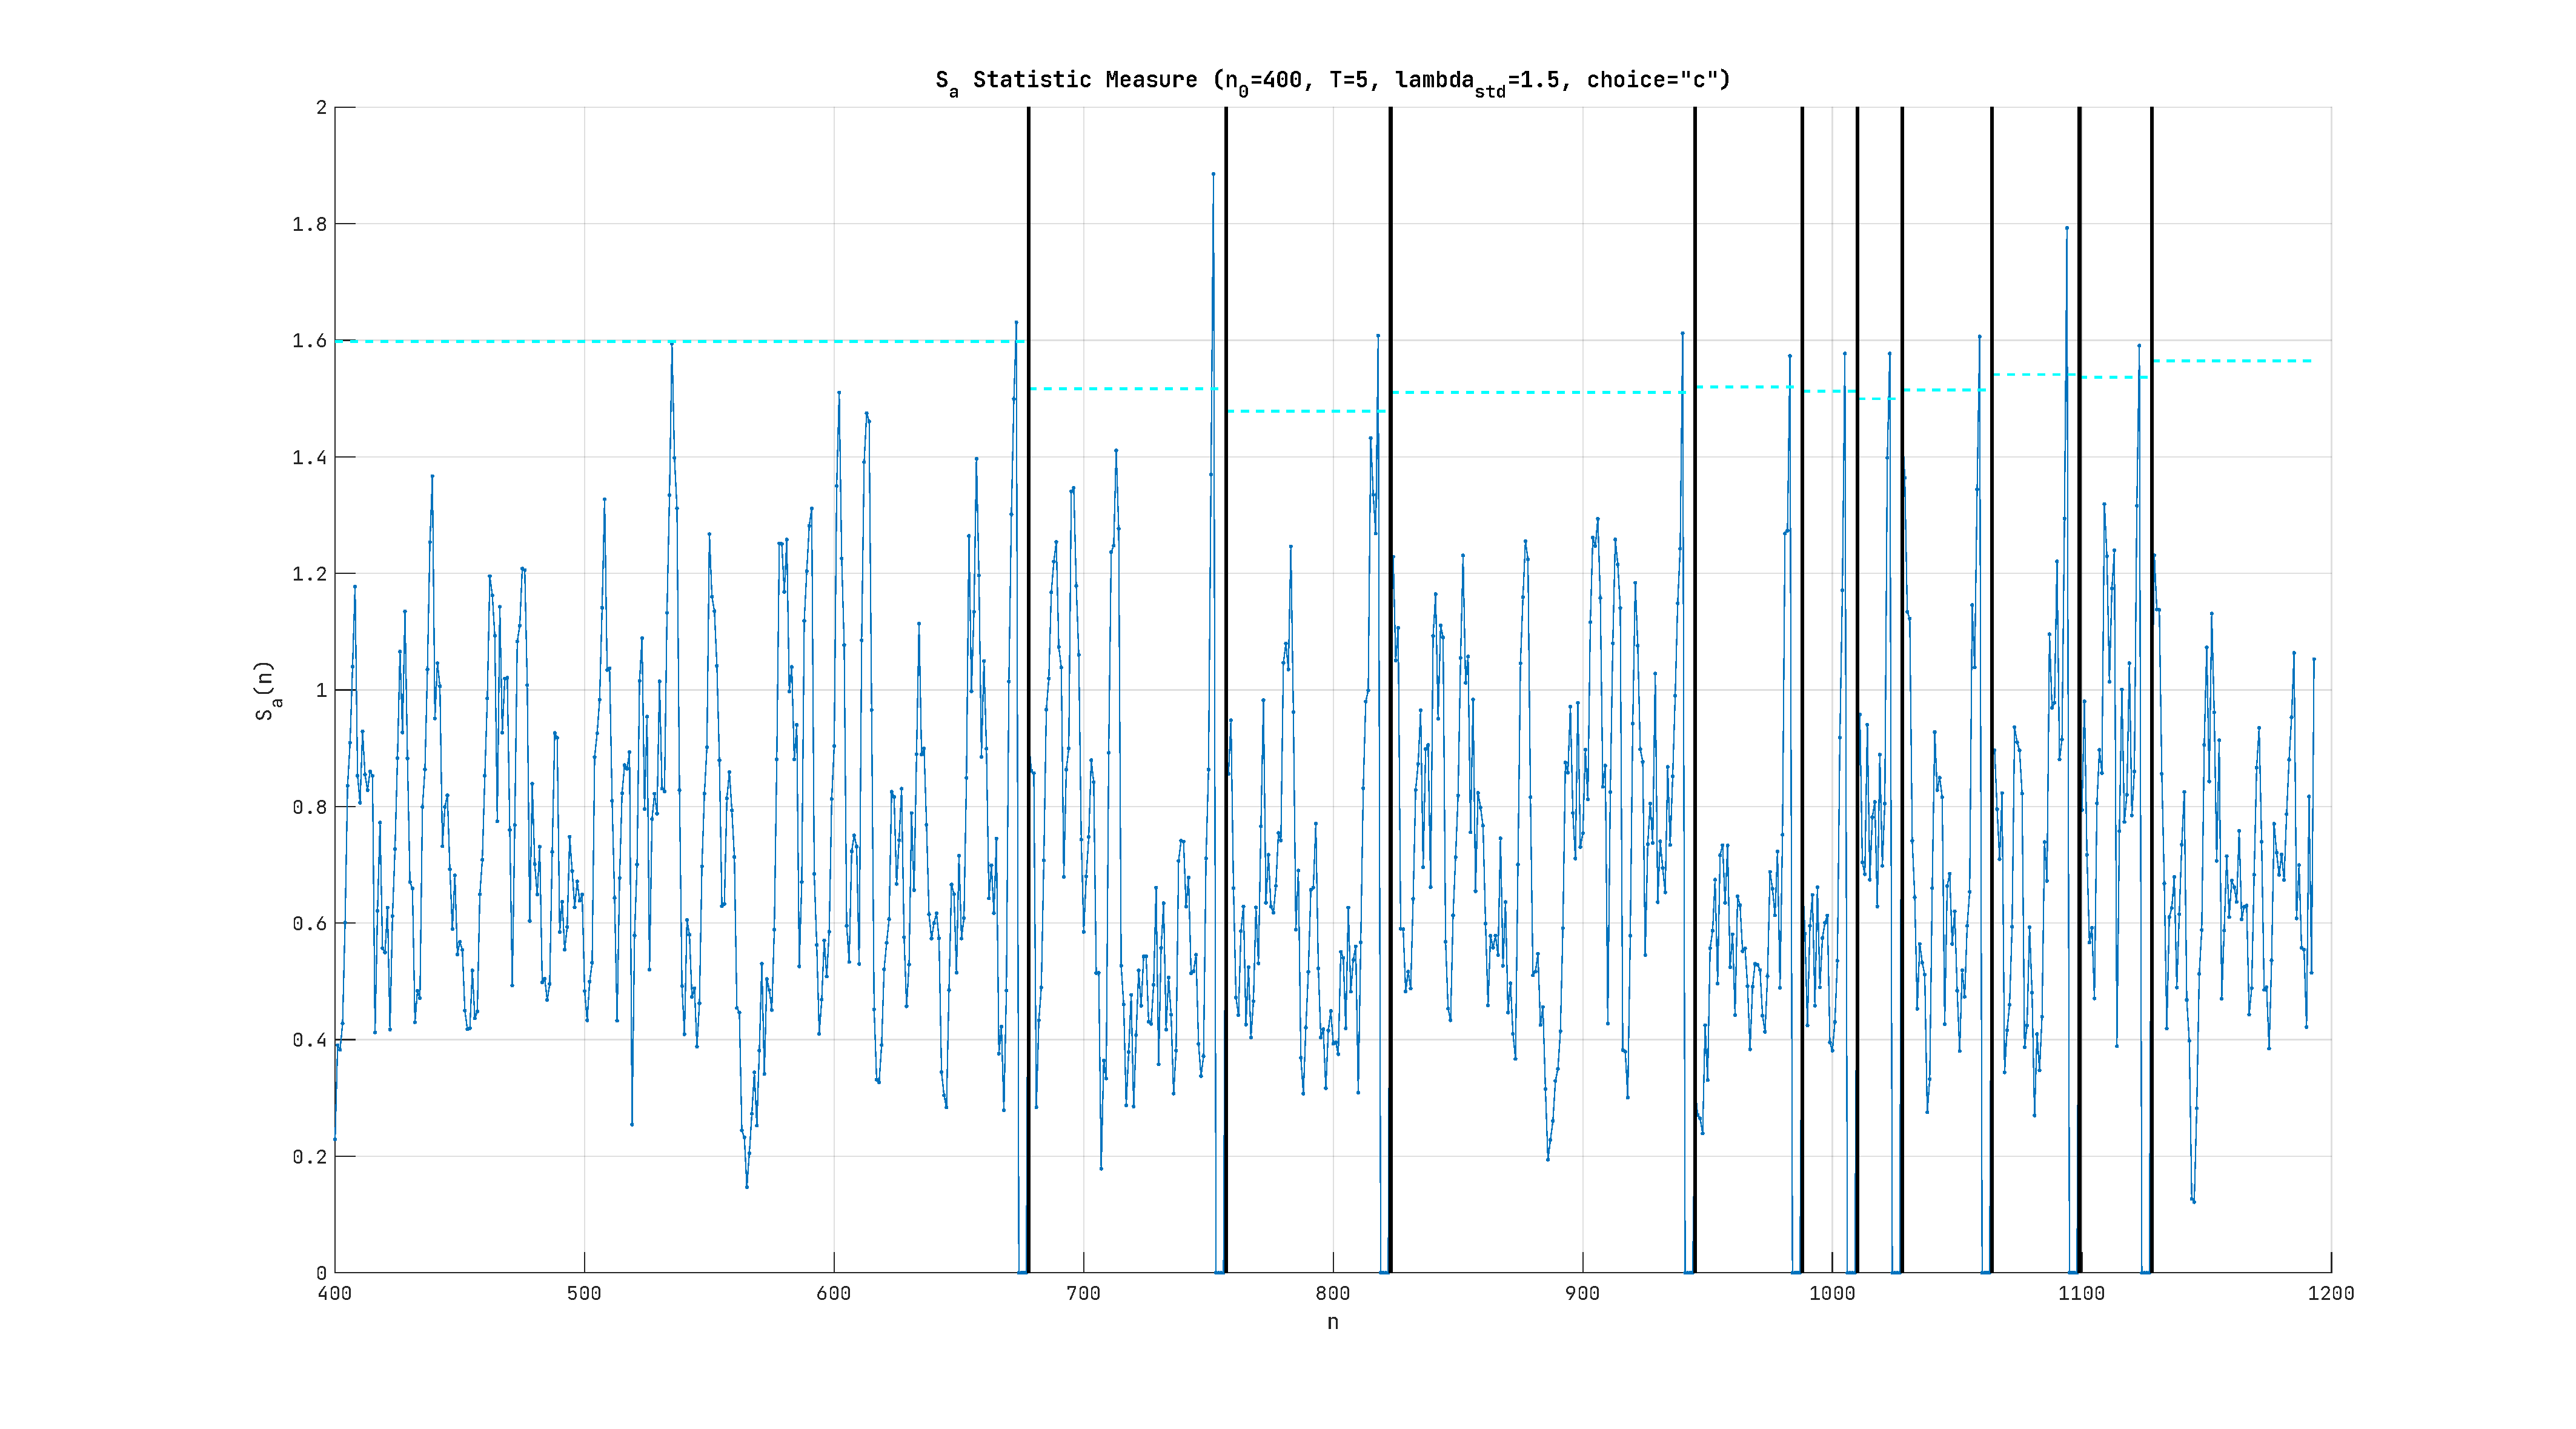
\includegraphics[width=\textwidth]{plots/mcps_xa.svg.pdf}
        \caption{Τιμές στατιστικού $S_n$ για έως και 5 βήματα μπροστά πρόβλεψη με $MA(1)$ της στάσιμης χρονοσειράς $\{X_a(t)\}$. Σημειώνονται επίσης το κριτήριο απόφασης, $\alpha$, (\tl{cyan}) και φυσικά τα σημεία αλλαγής με έντονες κάθετες γραμμές στα εκάστοτε σημεία $n+T$ (μαύρο). Το $n$ ξεκινάει από το 400 και άρα το $S_n$ δεν ορίζεται για τιμές $n<n_0=400$.}
        \label{fig:mcps_xa}
    \end{center}
\end{figure}

Όπως φαίνεται στο παραπάνω διάγραμμα, επειδή έχει χρησιμοποιηθεί η επιλογή \textquote{\tl{c}} για την αναπροσαρμογή του μοντέλου, κάθε φορά που εντοπίζεται σημείο αλλαγής το μοντέλο επανεκτιμάται σε νέο \tl{training set} (που είναι οι τελευταίες 400 παρατηρήσεις από τη στιγμή $n+5$) και άρα αλλάζει η δειγματική τυπική απόκλιση των παρατηρήσεων του \tl{training set}. Αυτό φαίνεται ως αλλαγή στο επίπεδο της \tl{cyan} διακεκομμένης γραμμής. 

\par Παρακάτω, τα ίδια σημεία αλλαγής απεικονίζονται στην αρχική χρονοσειρά προβολών του βίντεο \tl{A} και κατόπιν ακολουθεί σύντομος σχολιασμός:

\begin{figure}[H]
    \begin{center}
        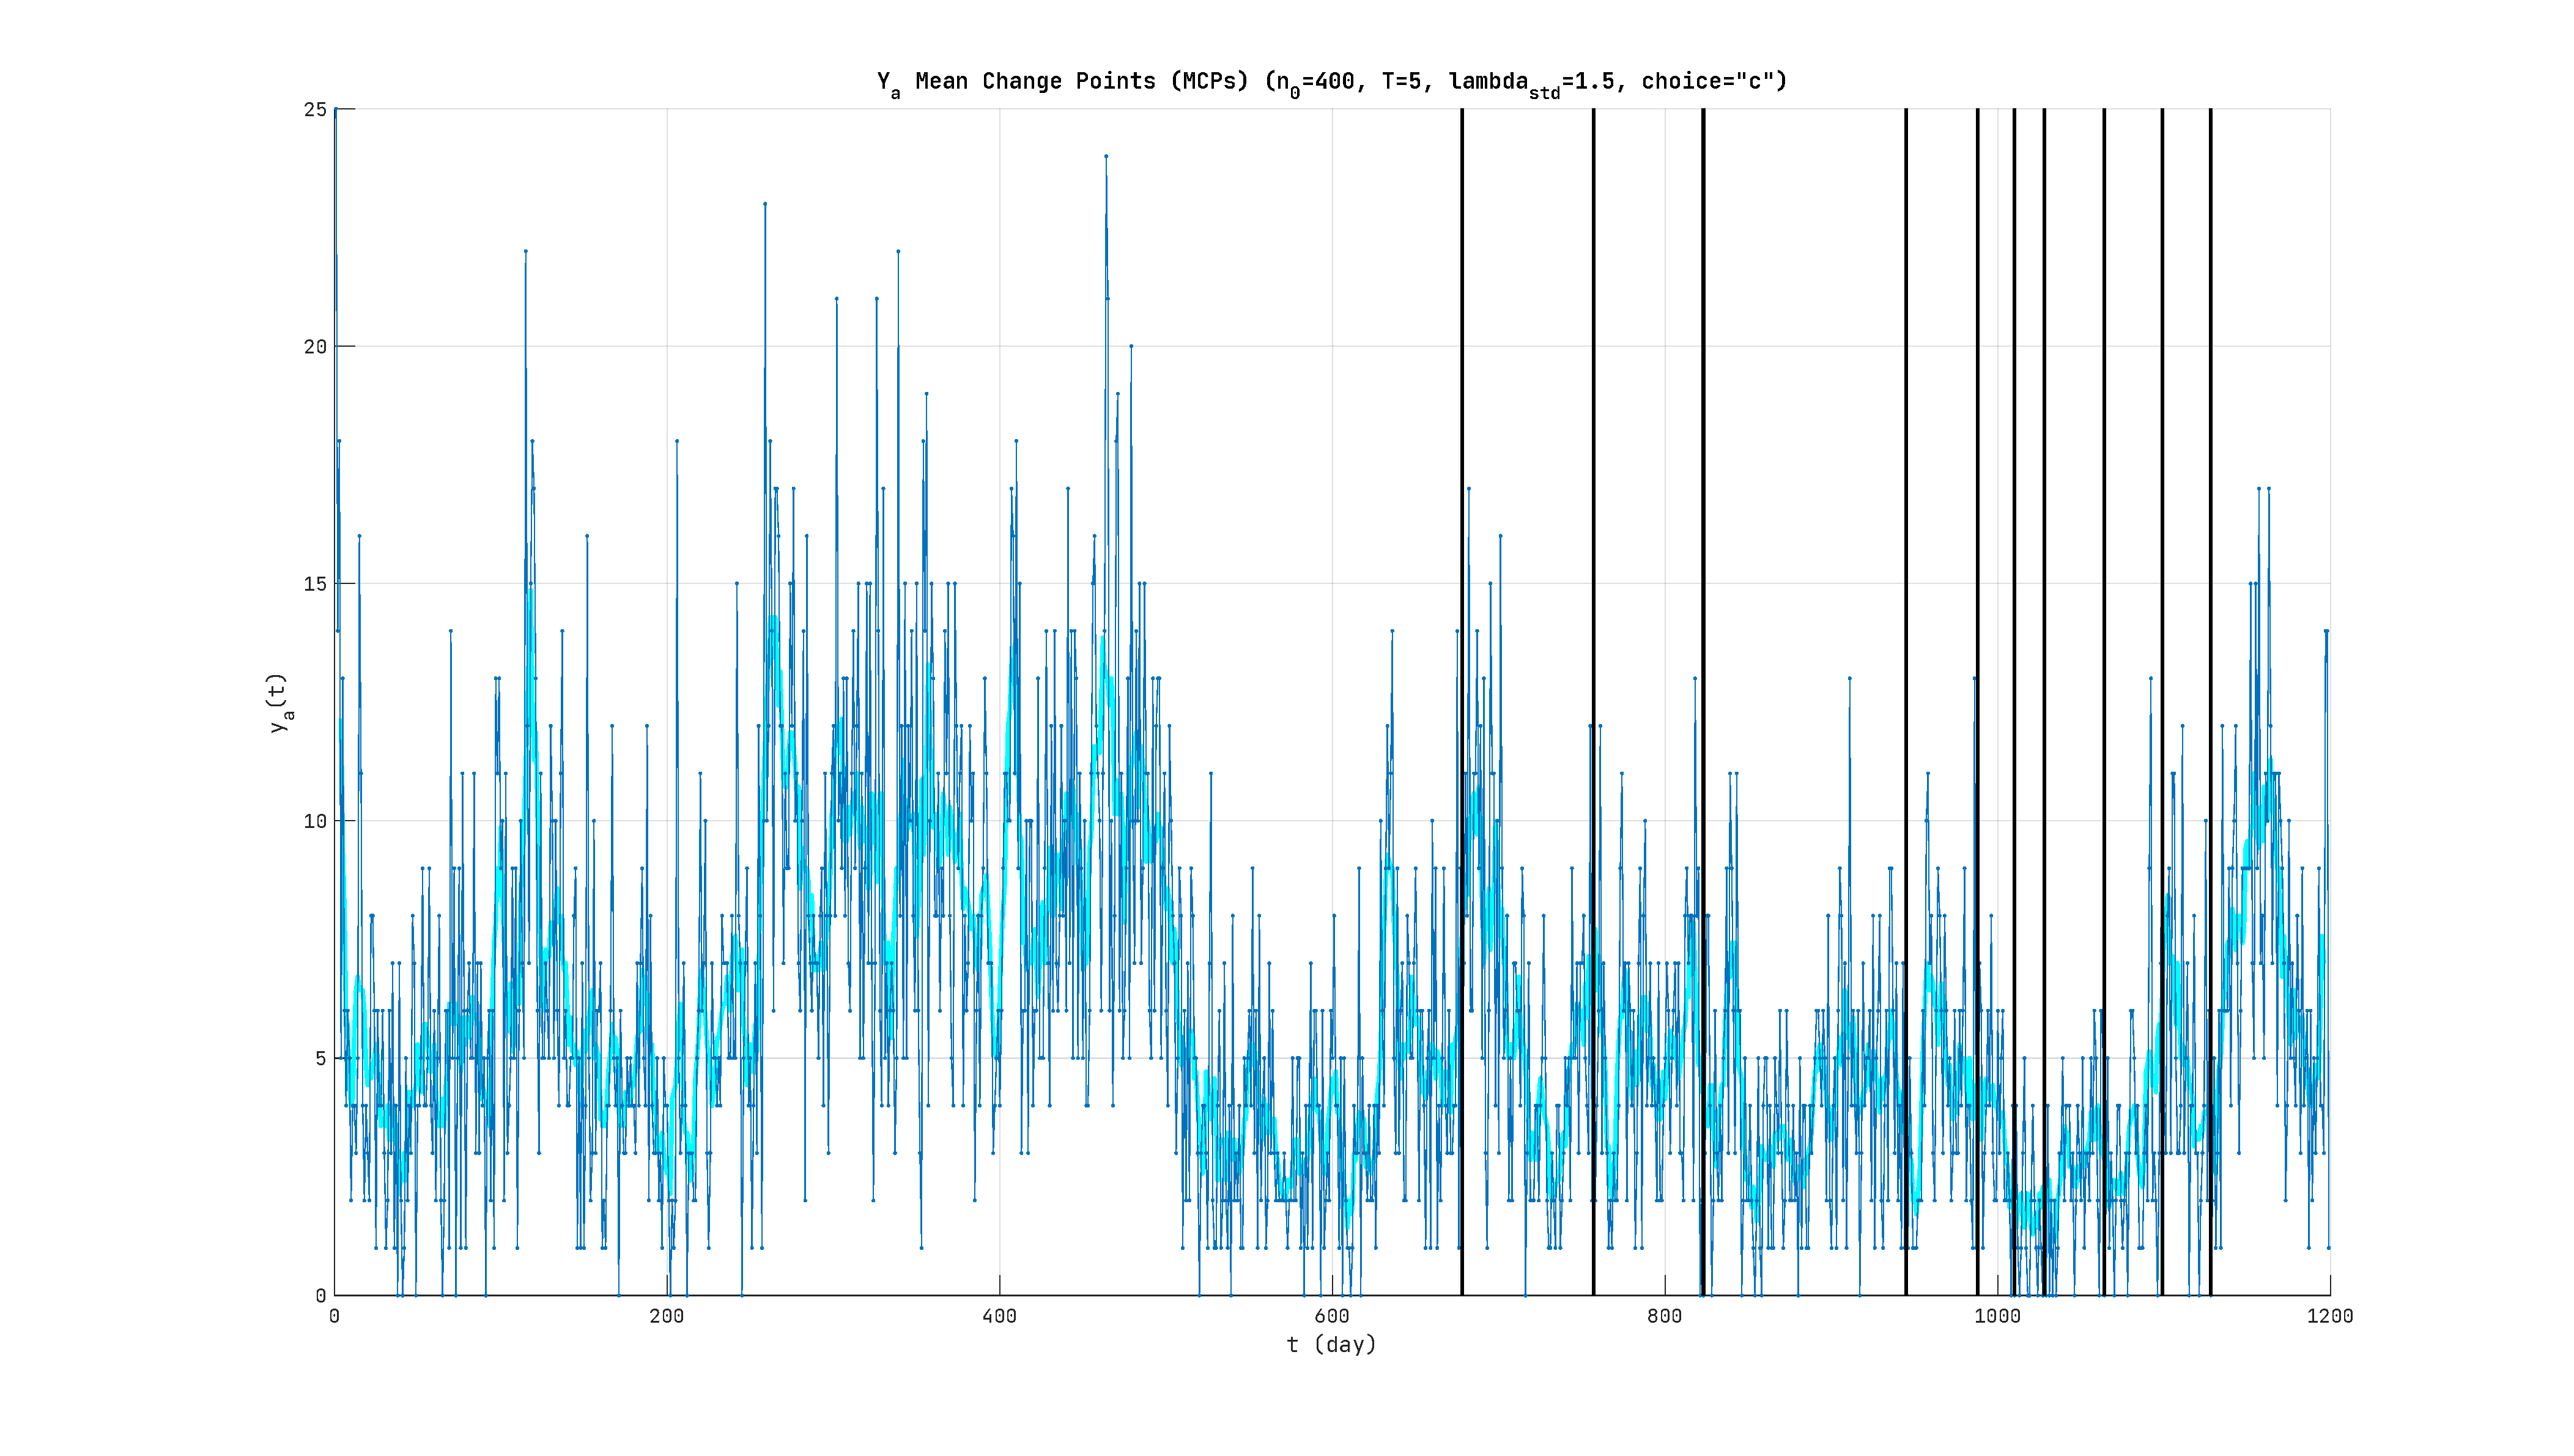
\includegraphics[width=\textwidth]{plots/mcps_ya.svg.pdf}
        \caption{Διάγραμμα ιστορίας της αρχικής χρονοσειράς $\{Y_a(t)\}$ (μπλε) μαζί με τα σημεία αλλαγής (μαύρο) που επιλέχθηκαν από την ανάλυση της στάσιμης εκδοχής της, καθώς και εκτίμηση της τάσης με φίλτρο κινούμενου μέσου τάξης 7 ($MA(7)$ \tl{smoothing})}
        \label{fig:mcps_ya}
    \end{center}
\end{figure}

Βλέποντας το πού \textquote{πέφτουν} τα σημεία αλλαγής στην αρχική χρονοσειρά προβολών του βιντέο \tl{A} παρατηρούμε πως αυτά δεν είναι σε τυχαίες θέσεις. Βρίσκοντα είτε σε κορυφές, δηλαδή σε θέσεις που αριστερά υπάρχει τοπικά αυξητική τάση και δεξιά τοπικά πτωτική (ακόμα και εάν αυτό γίνεται για λίγες παρατηρήσεις), ή σε βυθούς, δηλαδή σε σημεία που αριστερά υπάρχει τοπικά πτωτική τάση ενώ δεξία αυτή αλλάζει και γίνεται αυξυτική. Είναι κάπως λογικό οι προβλέψεις μας για τις γειτονιές τέτοιων σημείων (ακόμα και εάν γίνονται μέσω στάσιμων εκδοχών των αρχικών χρονοσειρών) με γραμμικά μοντέλα να εμφανίζουν αρκετά σημαντικά σφάλματα ώστε να σηματοδοτηθούν σημεία αλλαγής.

\par Ακολουθεί μια πιο ενδελεχής ανάλυση για την επιλογή των \tl{hyperparameters} που σε αυτήν την υποενότητα έγινε κάπως αυθαίρετα.

\section{Επιλογή Βέλτιστων Παραμέτρων}

Για επιλογή βέλτιστων τιμών στις \tl{hyperparameters} της μεθόδου και συγκεκριμένα στον ορίζοντα πρόβλεψης, $T$, και στο $\lambda_{std}$ του ορίου απόφασης, $\alpha$, θα κάνουμε αναζήτηση πλέγματος ως προς αυτές. Ως μετρικές για αξιολόγηση του κάθε συνδυασμού των παραμέτρων αυτών χρησιμοποιήθηκαν οι εξής δύο (2):
\begin{itemize}
    \item \textit{Αριθμός \tl{MCPs}}: Θέλουμε ο αριθμός των σημείων αλλαγής (\tl{MCPs}) να μην είναι πολύ μεγάλος καθώς κάτι τέτοιο κάνει λιγότερο αξιόπιστη την όλη μέθοδο, αλλά να μην είναι και πολύ μικρός ώστε να υπάρχει νόημα χρήσης της μεθόδου (π.χ. αν έβγαζε ένα ή δύο σημεία αλλαγής τότε μάλλον δεν θα άξιζε η \tl{on-line} χρήση της μεθόδου για πρόβλεψη αλλαγών της ζήτησης σε εφαρμογές όπως αυτή του δοθέντος \tl{paper})
    \item \textit{\tl{NRMSE} Προβλέψεων}: Σε αυτή τη μετρική υπολογίζουμε το \tl{NRMSE} μεταξύ των προβλέψεων που χρησιμοποίηθηκαν για τον εντοπισμό των σημείων αλλαγής και των πραγματικών τιμών της στάσιμης χρονοσειράς
\end{itemize}

Αρχικά παραθέτονται σε διαγράμματα τύπου \tl{surf} τα αποτελέσματα αναζήτησης πλέγματος ως προς τις παραπάνω μετρικές ενώ στη συνέχεια σχολιάζεται ο τρόπος επιλογής προσεγγεστικά βέλτιστων παραμάτρων αλλά και οι τελικές τους τιμές.

\begin{figure}[H]
    \begin{center}
        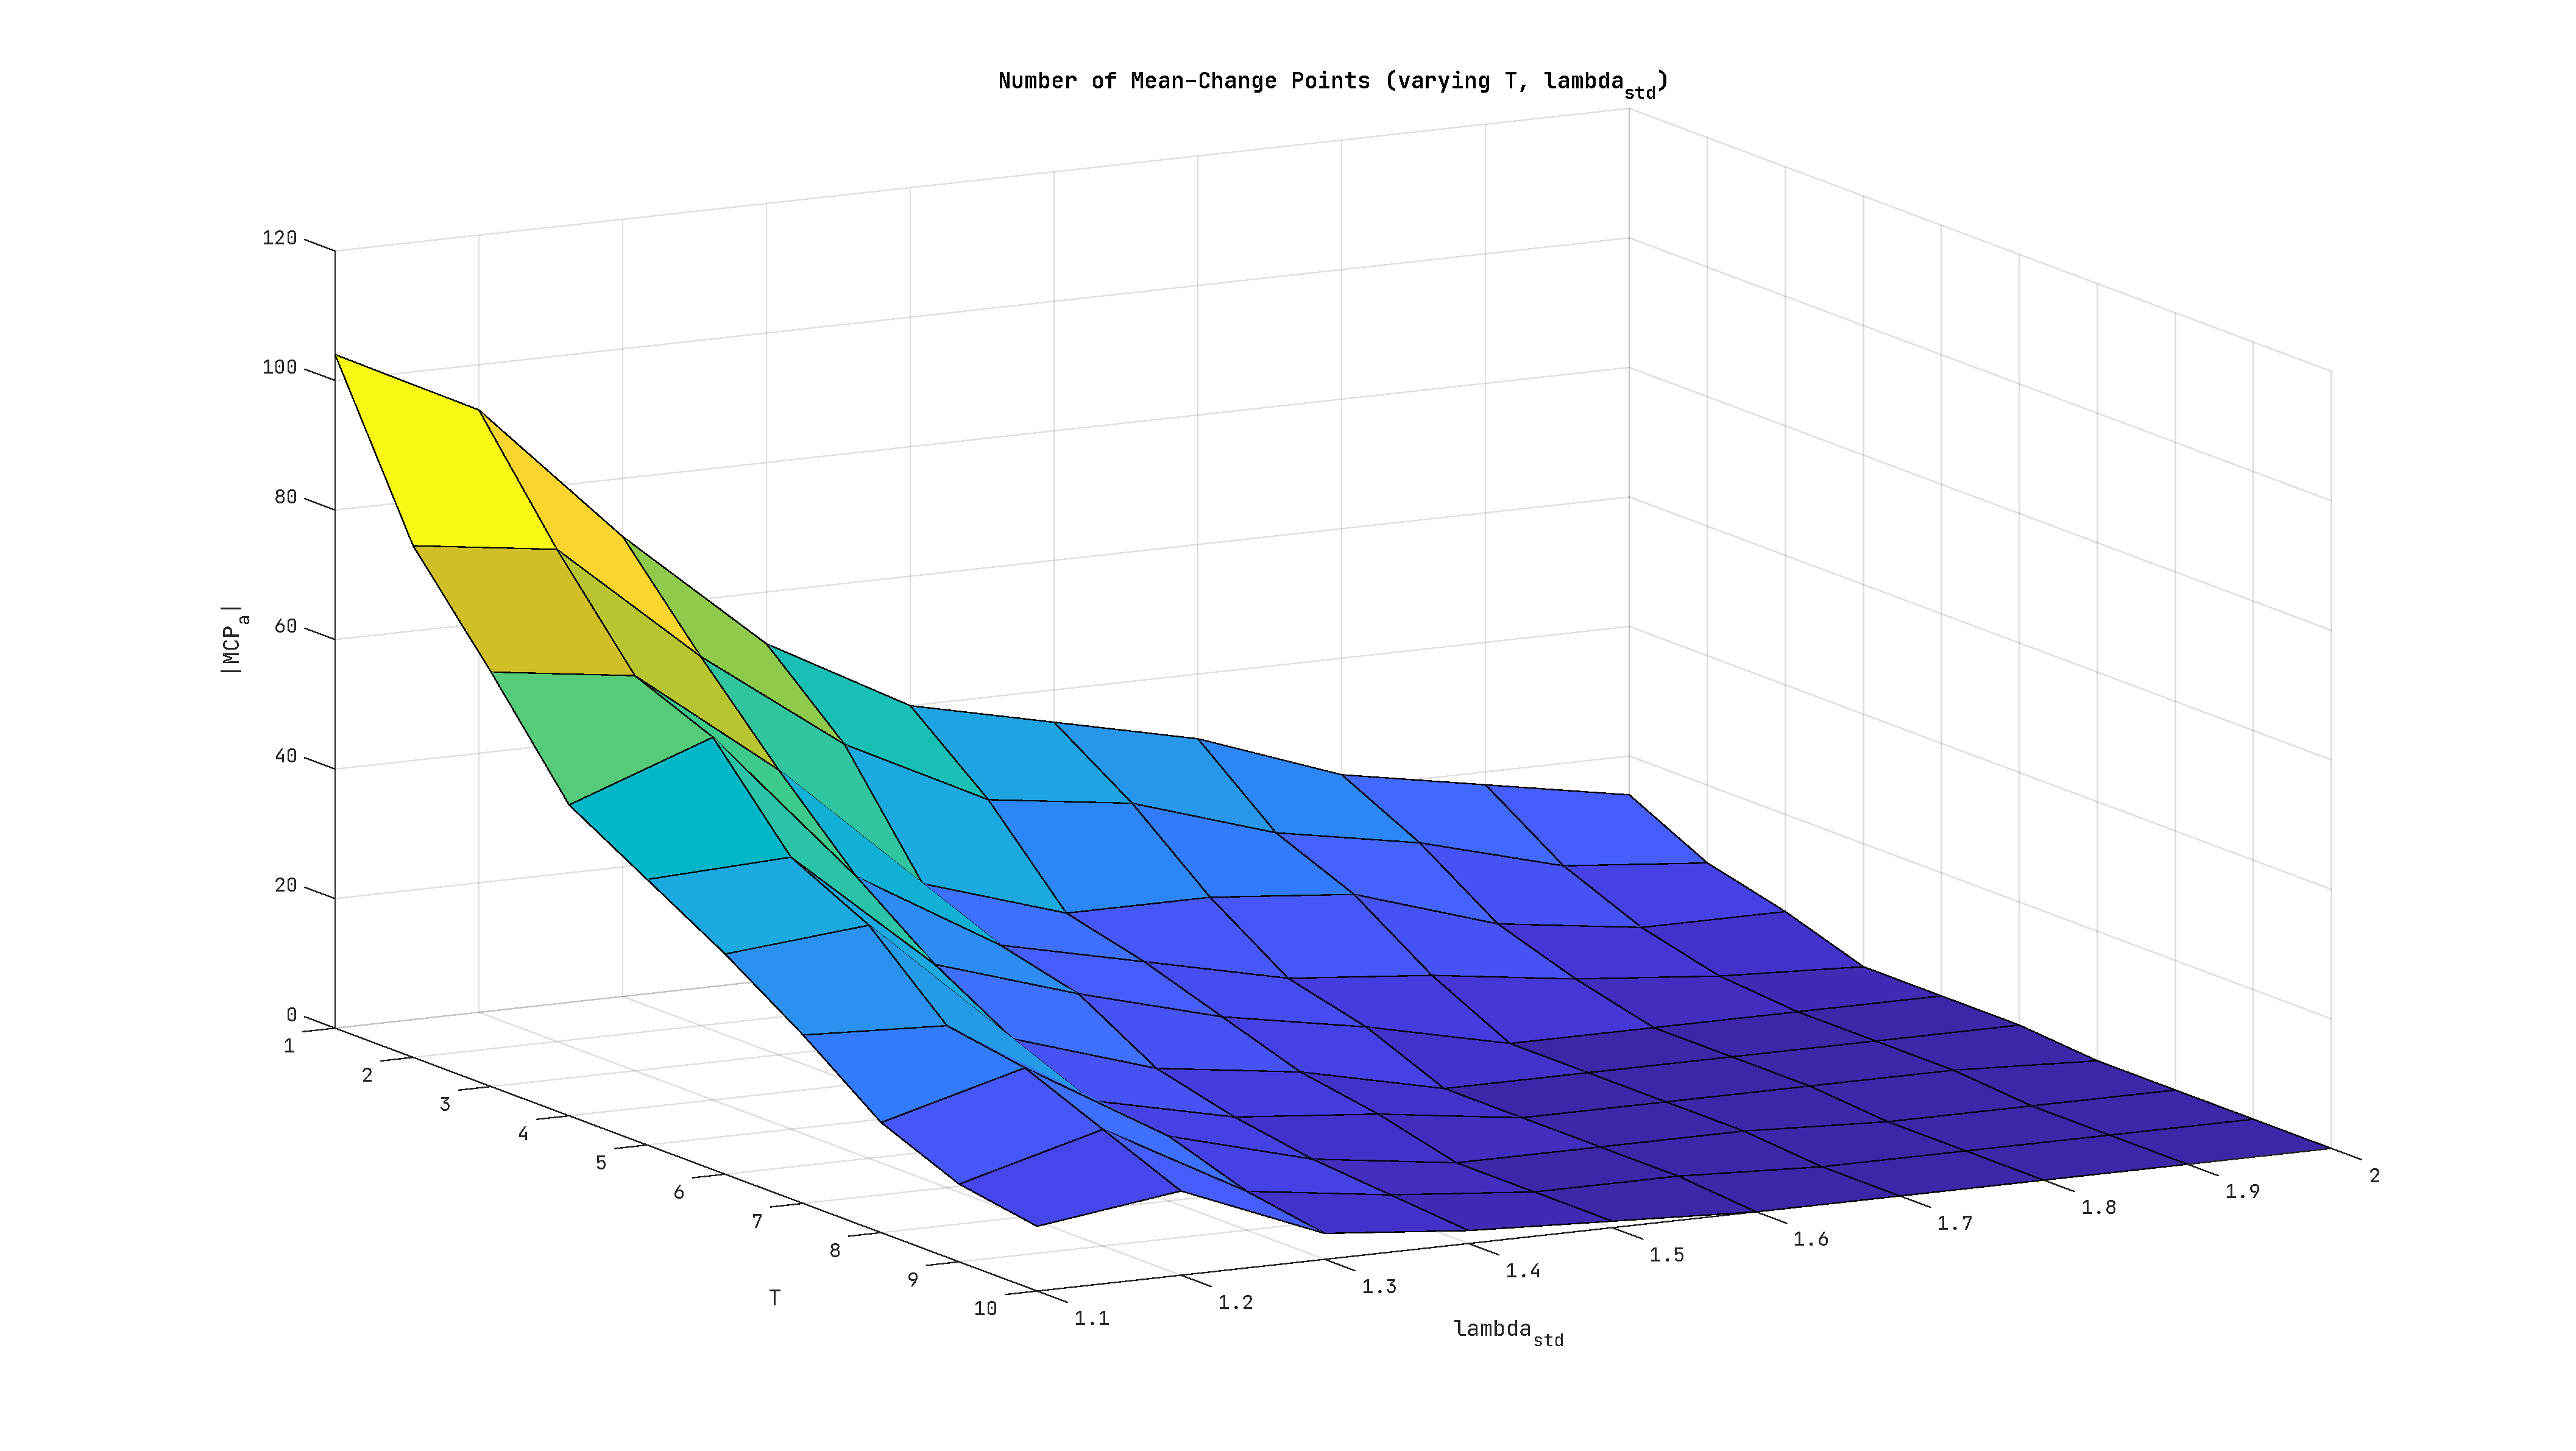
\includegraphics[width=\textwidth]{plots/mcps_count_a.svg.pdf}
        \caption{Αριθμός σημείων αλλαγής, $\vert$\tl{MCP}$\vert$, που προκύπτουν για κάθε τιμή του πλέγματος αναζήτησης ως πρός τον ορίζοντα πρόβλεψης, $T$, και το $\lambda_{std}$ του ορίου απόφασης, $\alpha$}
        \label{fig:mcps_count_a}
    \end{center}
\end{figure}

\begin{figure}[H]
    \begin{center}
        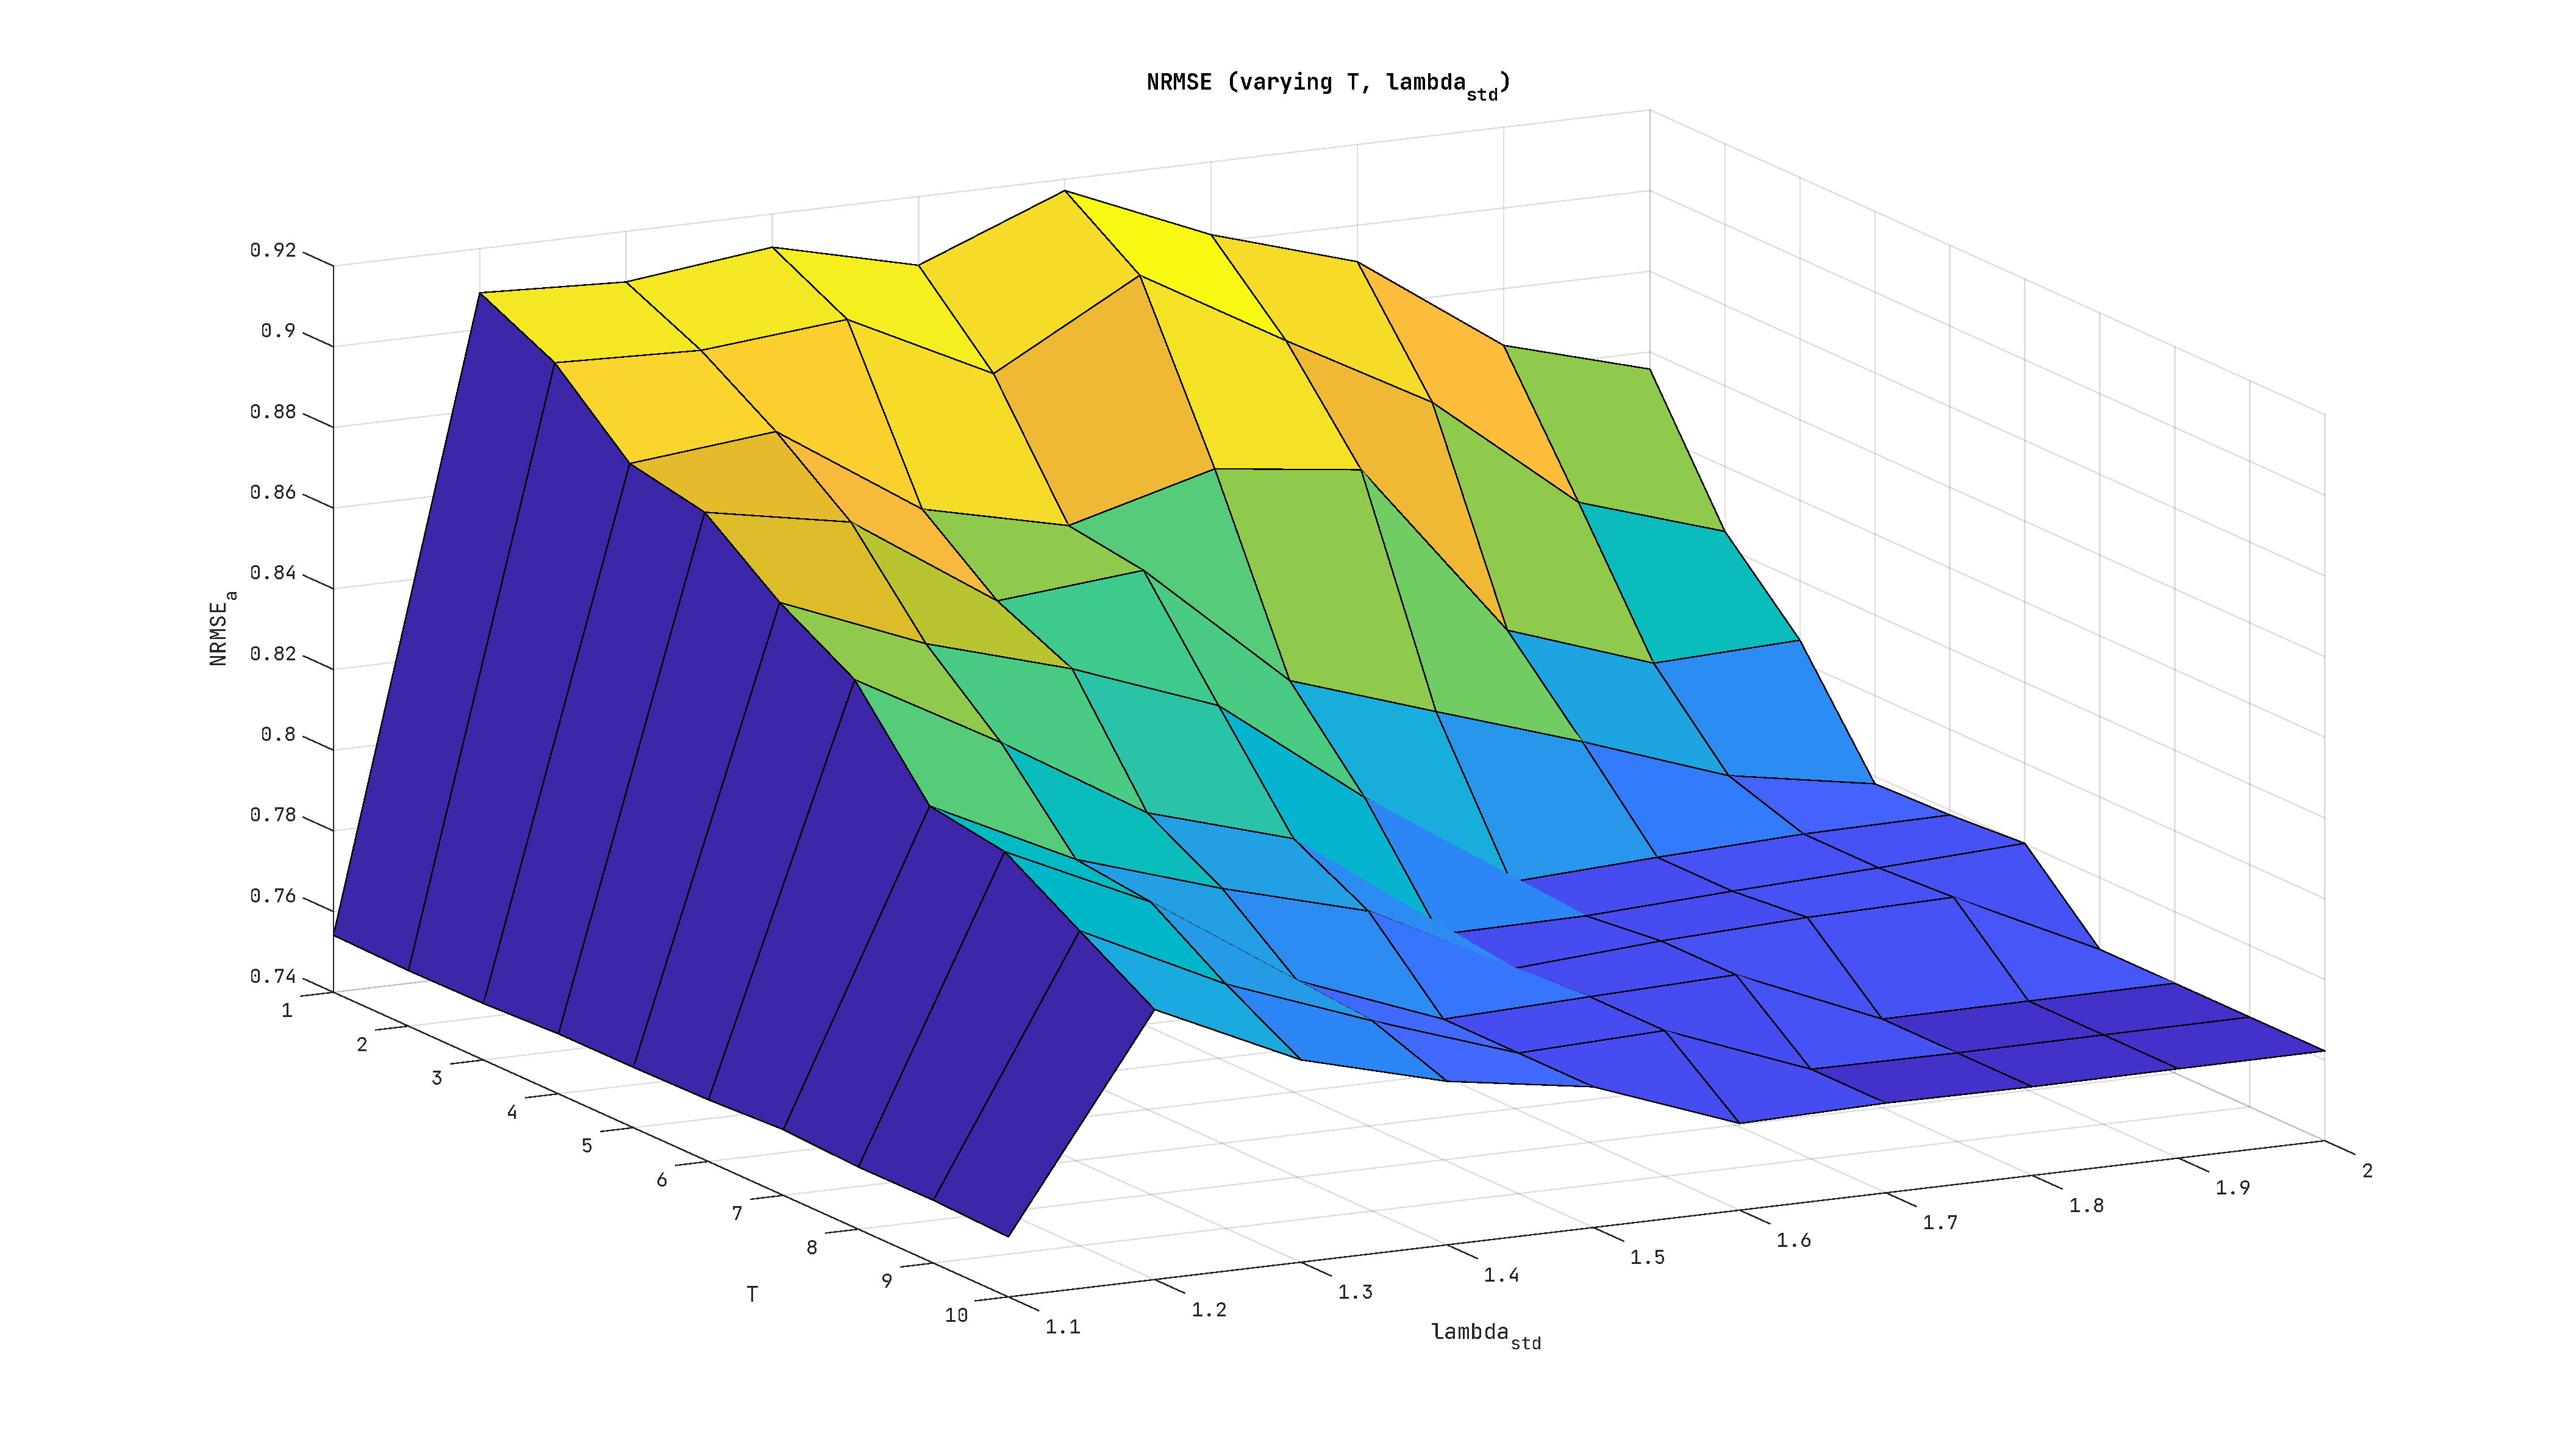
\includegraphics[width=\textwidth]{plots/nrmse_a.svg.pdf}
        \caption{\tl{NRMSE} προβλέψεων κατά τον υπολογισμό των σημείων αλλαγής (\tl{MCPs}), για κάθε τιμή του πλέγματος αναζήτησης ως πρός τον ορίζοντα πρόβλεψης, $T$, και το $\lambda_{std}$ του ορίου απόφασης, $\alpha$}
        \label{fig:nrmse_a}
    \end{center}
\end{figure}

\par Γενικότερα, αναζητούμε τα \textquote{γόνατα} στις αντίστοιχες τρισδιάστατες καμπύλες έτσι ώστε περαιτέρω μεταβολές των αντίστοιχων παραμέτρων να μην είναι πλέον επικερδείς.

\par Επικεντρώνοντας στο πρώτο διάγραμμα και δεδομένου ότι θέλουμε ο αριθμός των \tl{MCPs} να μήν είναι πολύ μεγάλος ή πολύ μικρός, θα επιλέγαμε τις ακόλουθες τιμές (προσεγγιστικά):
\begin{align}
    T \in [5,8] \ \ \ \& \ \ \ \lambda_{std} \in [1.3, 1.6]
    \label{eq:t_lambda_mcps_a}
\end{align}

\par Επικεντρώνοντας τώρα στο διάγραμμα των \tl{NRMSEs} και δεδομένου ότι θέλουμε το \tl{NRMSE} να είναι κατά το δυνατό μικρό, θα επιλέγαμε τις ακόλουθες τιμές (προσεγγιστικά):
\begin{align}
    T \geq 6 \ \ \ \& \ \ \ \lambda_{std} \geq 1.5
    \label{eq:t_lambda_nrmses_a}
\end{align}

\par Συνδυάζοντας τις σχέσεις (\ref{eq:t_lambda_mcps_a}) και (\ref{eq:t_lambda_nrmses_a}) παραπάνω καταλήγουμε ότι οι \tl{hyperparameters} που θα χρησιμοποιηθούν για την εφαρμογή της μεθόδου αυτόματης εύρεσης χρονικών σημείων αλλαγής θα είναι:
\textbf{T = 6 βήματα} και \textbf{λ\textsubscript{\tl{std}} = 1.5}. Οι αντίστοιχες τιμές του \tl{grid search} είναι: \textbf{$\vert$\tl{MCP}$\vert$ = 6 \tl{MCPs}} και \textbf{\tl{NRMSE} = 0.8}.


\section{Εφαρμογή με Βέλτιστες Παραμέτρους}

Χρησιμοποιώντας τις επιλεγμένες τιμές για τις \tl{hyperparameters} της μεθόδου, δηλαδή ορίζοντα πρόβλεψης έως και 6 βημάτων εμπρός, $T=6$, και παράμετρο ορίου απόφασης στο 1.5, $\lambda_{std}=1.5$, θα τρέξουμε την παραπάνω μέθοδο στη στάσιμη χρονοσειρά που προέκυψε από το βήμα 2, $\{X_a(t)\}$, και στο $MA(1)$ μοντέλο που προσαρμόστηκε σε αυτή (σχέση \ref{eq:xa_model}). Παρακάτω, φαίνονται τα σημεία αλλαγής που προκύπτουν από την εκτέλεση της μεθόδους με τις παραπάνω παραμέτρους για κάθε μια από τις επιλογές αναπροσαρμογής του μοντέλου (\textquote{\tl{a}}, \textquote{\tl{b}} ή \textquote{\tl{c}}).

\subsection{Αναπροσαρμογή όταν βρεθεί σημείο αλλαγής}

Επιλογή \textquote{\tl{c}}

\begin{figure}[H]
    \begin{center}
        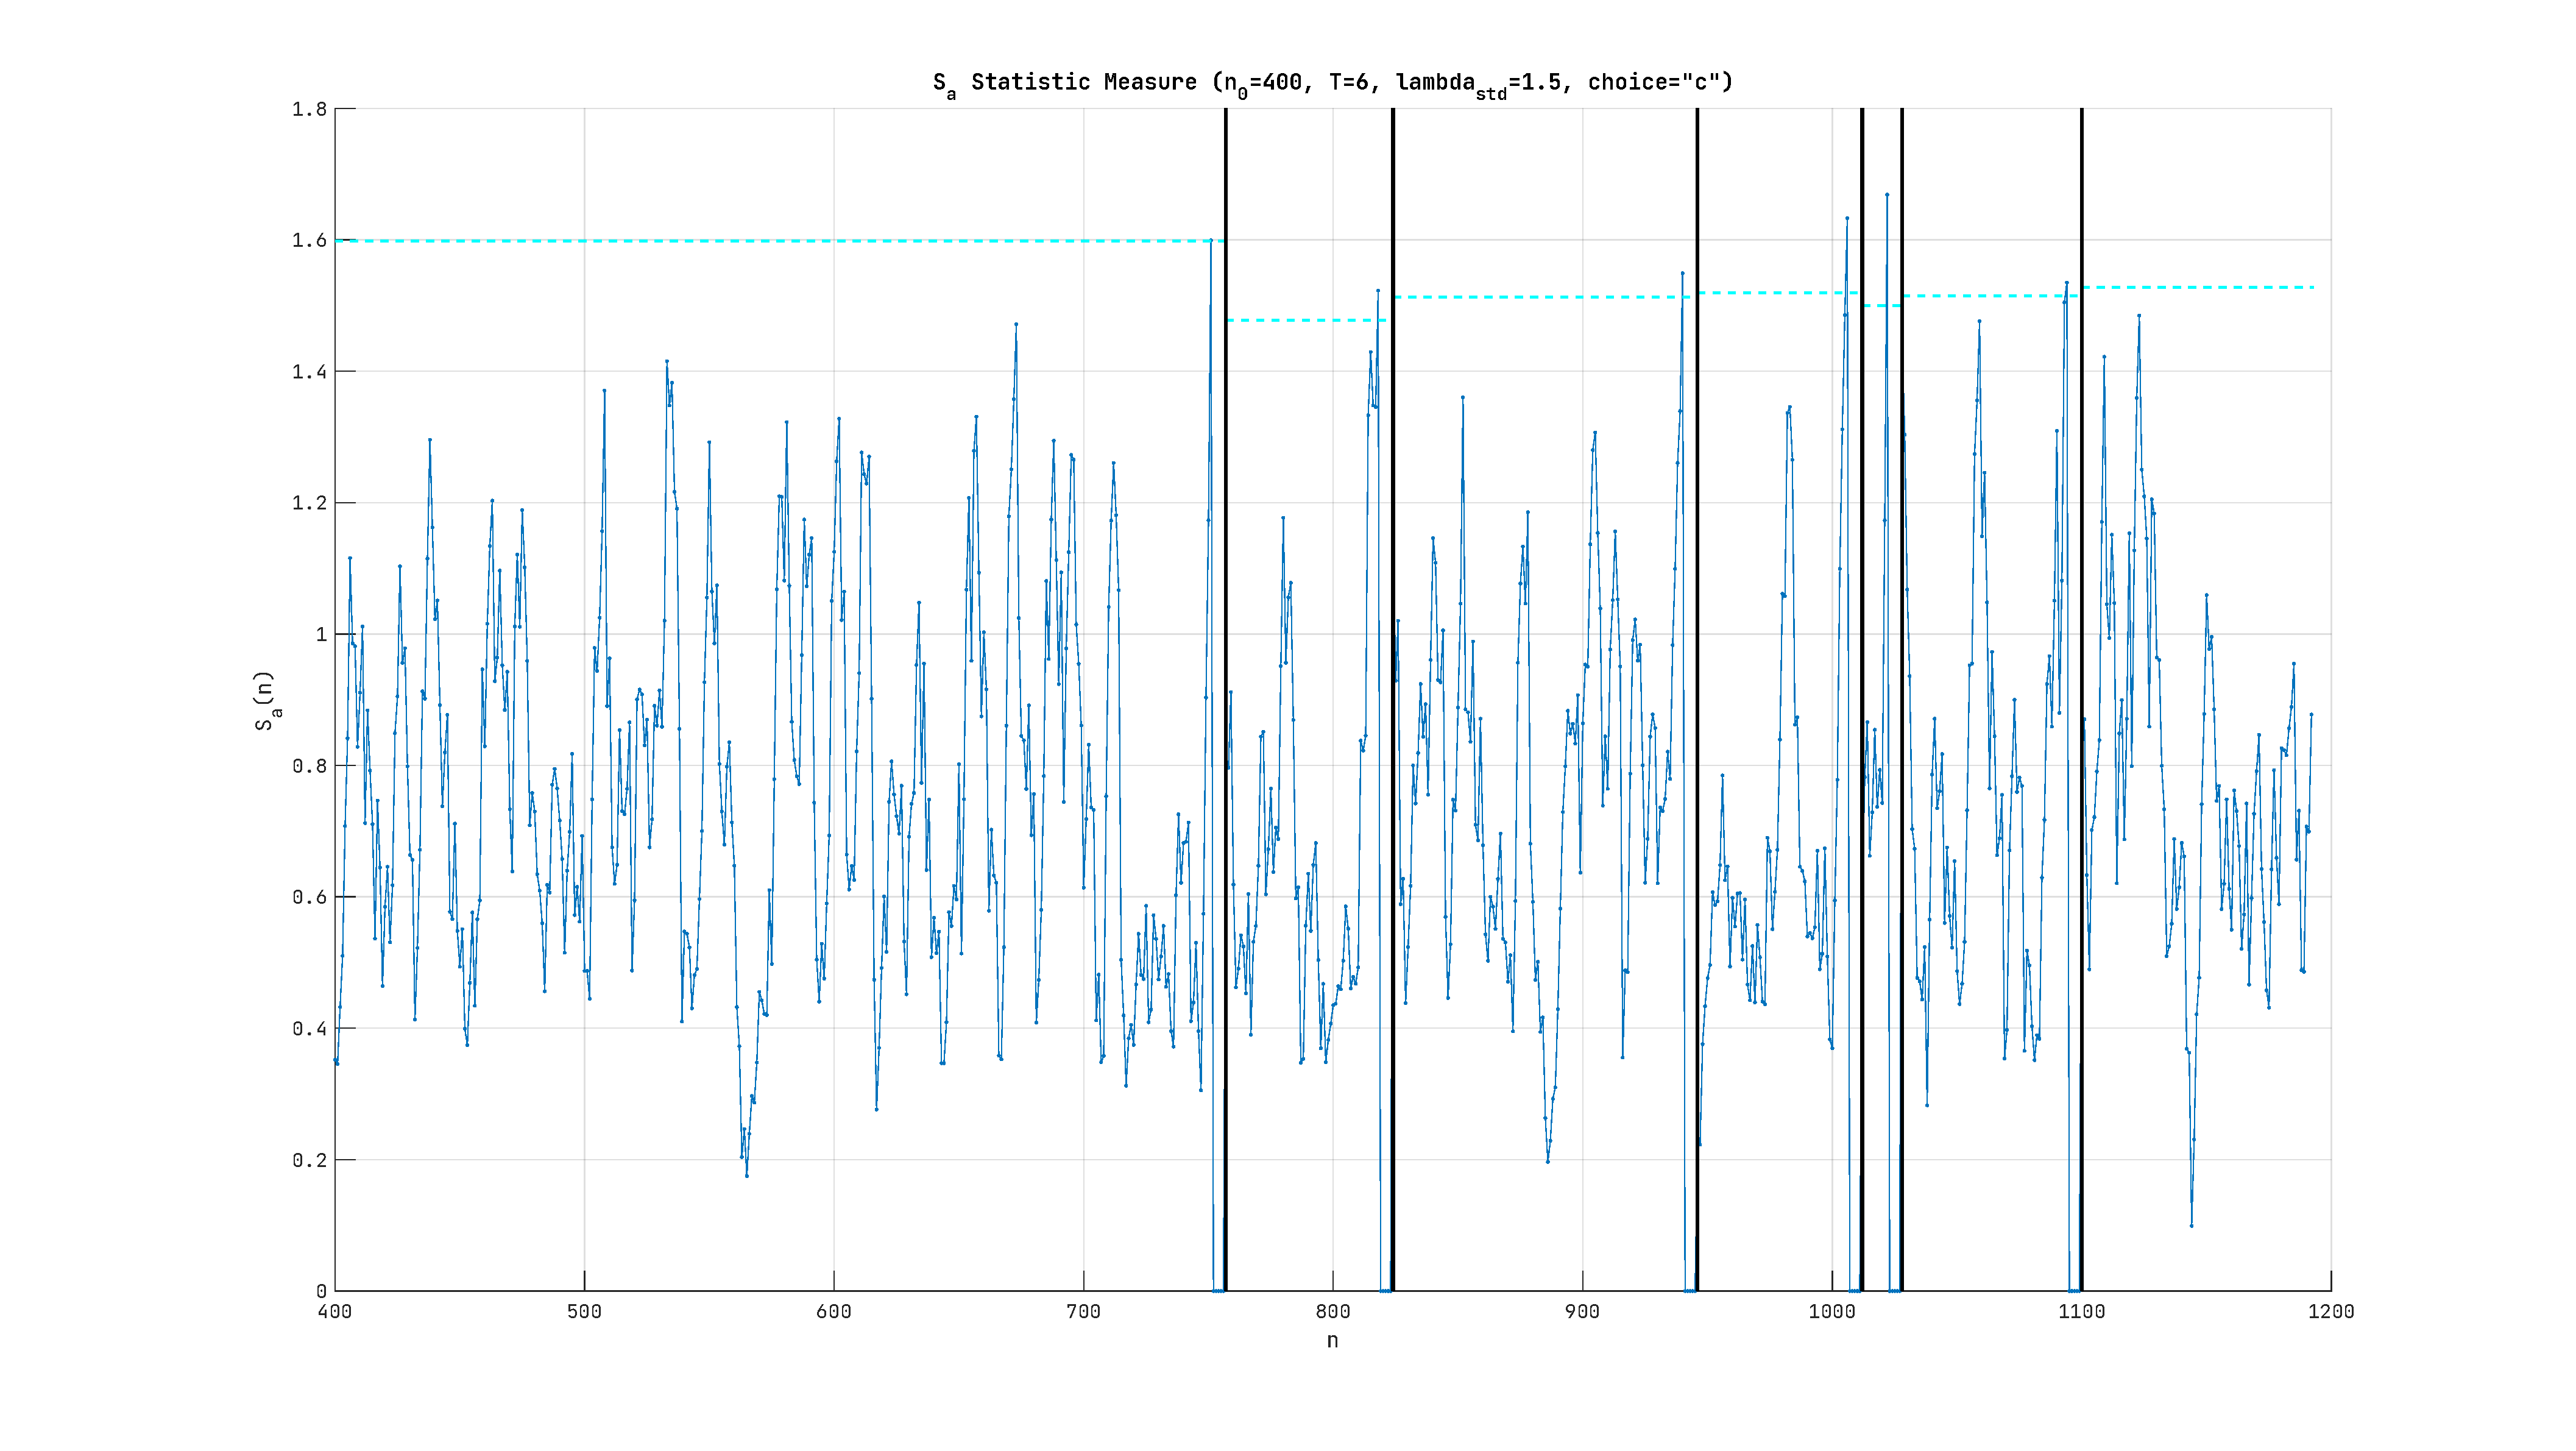
\includegraphics[width=\textwidth]{plots/mcps_xa_opt_c.svg.pdf}
        \caption{Τιμές στατιστικού $S_n$ για έως και 6 βήματα μπροστά πρόβλεψη με $MA(1)$ της στάσιμης χρονοσειράς $\{X_a(t)\}$ και για επιλογή αναπροσαρμογής \textquote{\tl{c}} (αναπροσαρμογή όταν βρεθεί σημείο αλλαγής). Σημειώνονται επίσης το κριτήριο απόφασης, $\alpha=1.5*s_x$, (\tl{cyan}) και φυσικά τα σημεία αλλαγής με έντονες κάθετες γραμμές στα εκάστοτε σημεία $n+T$ (μαύρο) - [\tl{NRMSE}=0.800, \ 28.9\tl{sec}]}
        \label{fig:mcps_xa_opt_c}
    \end{center}
\end{figure}

Παρακάτω, τα ίδια σημεία αλλαγής απεικονίζονται στην αρχική χρονοσειρά προβολών του βίντεο \tl{A}:

\begin{figure}[H]
    \begin{center}
        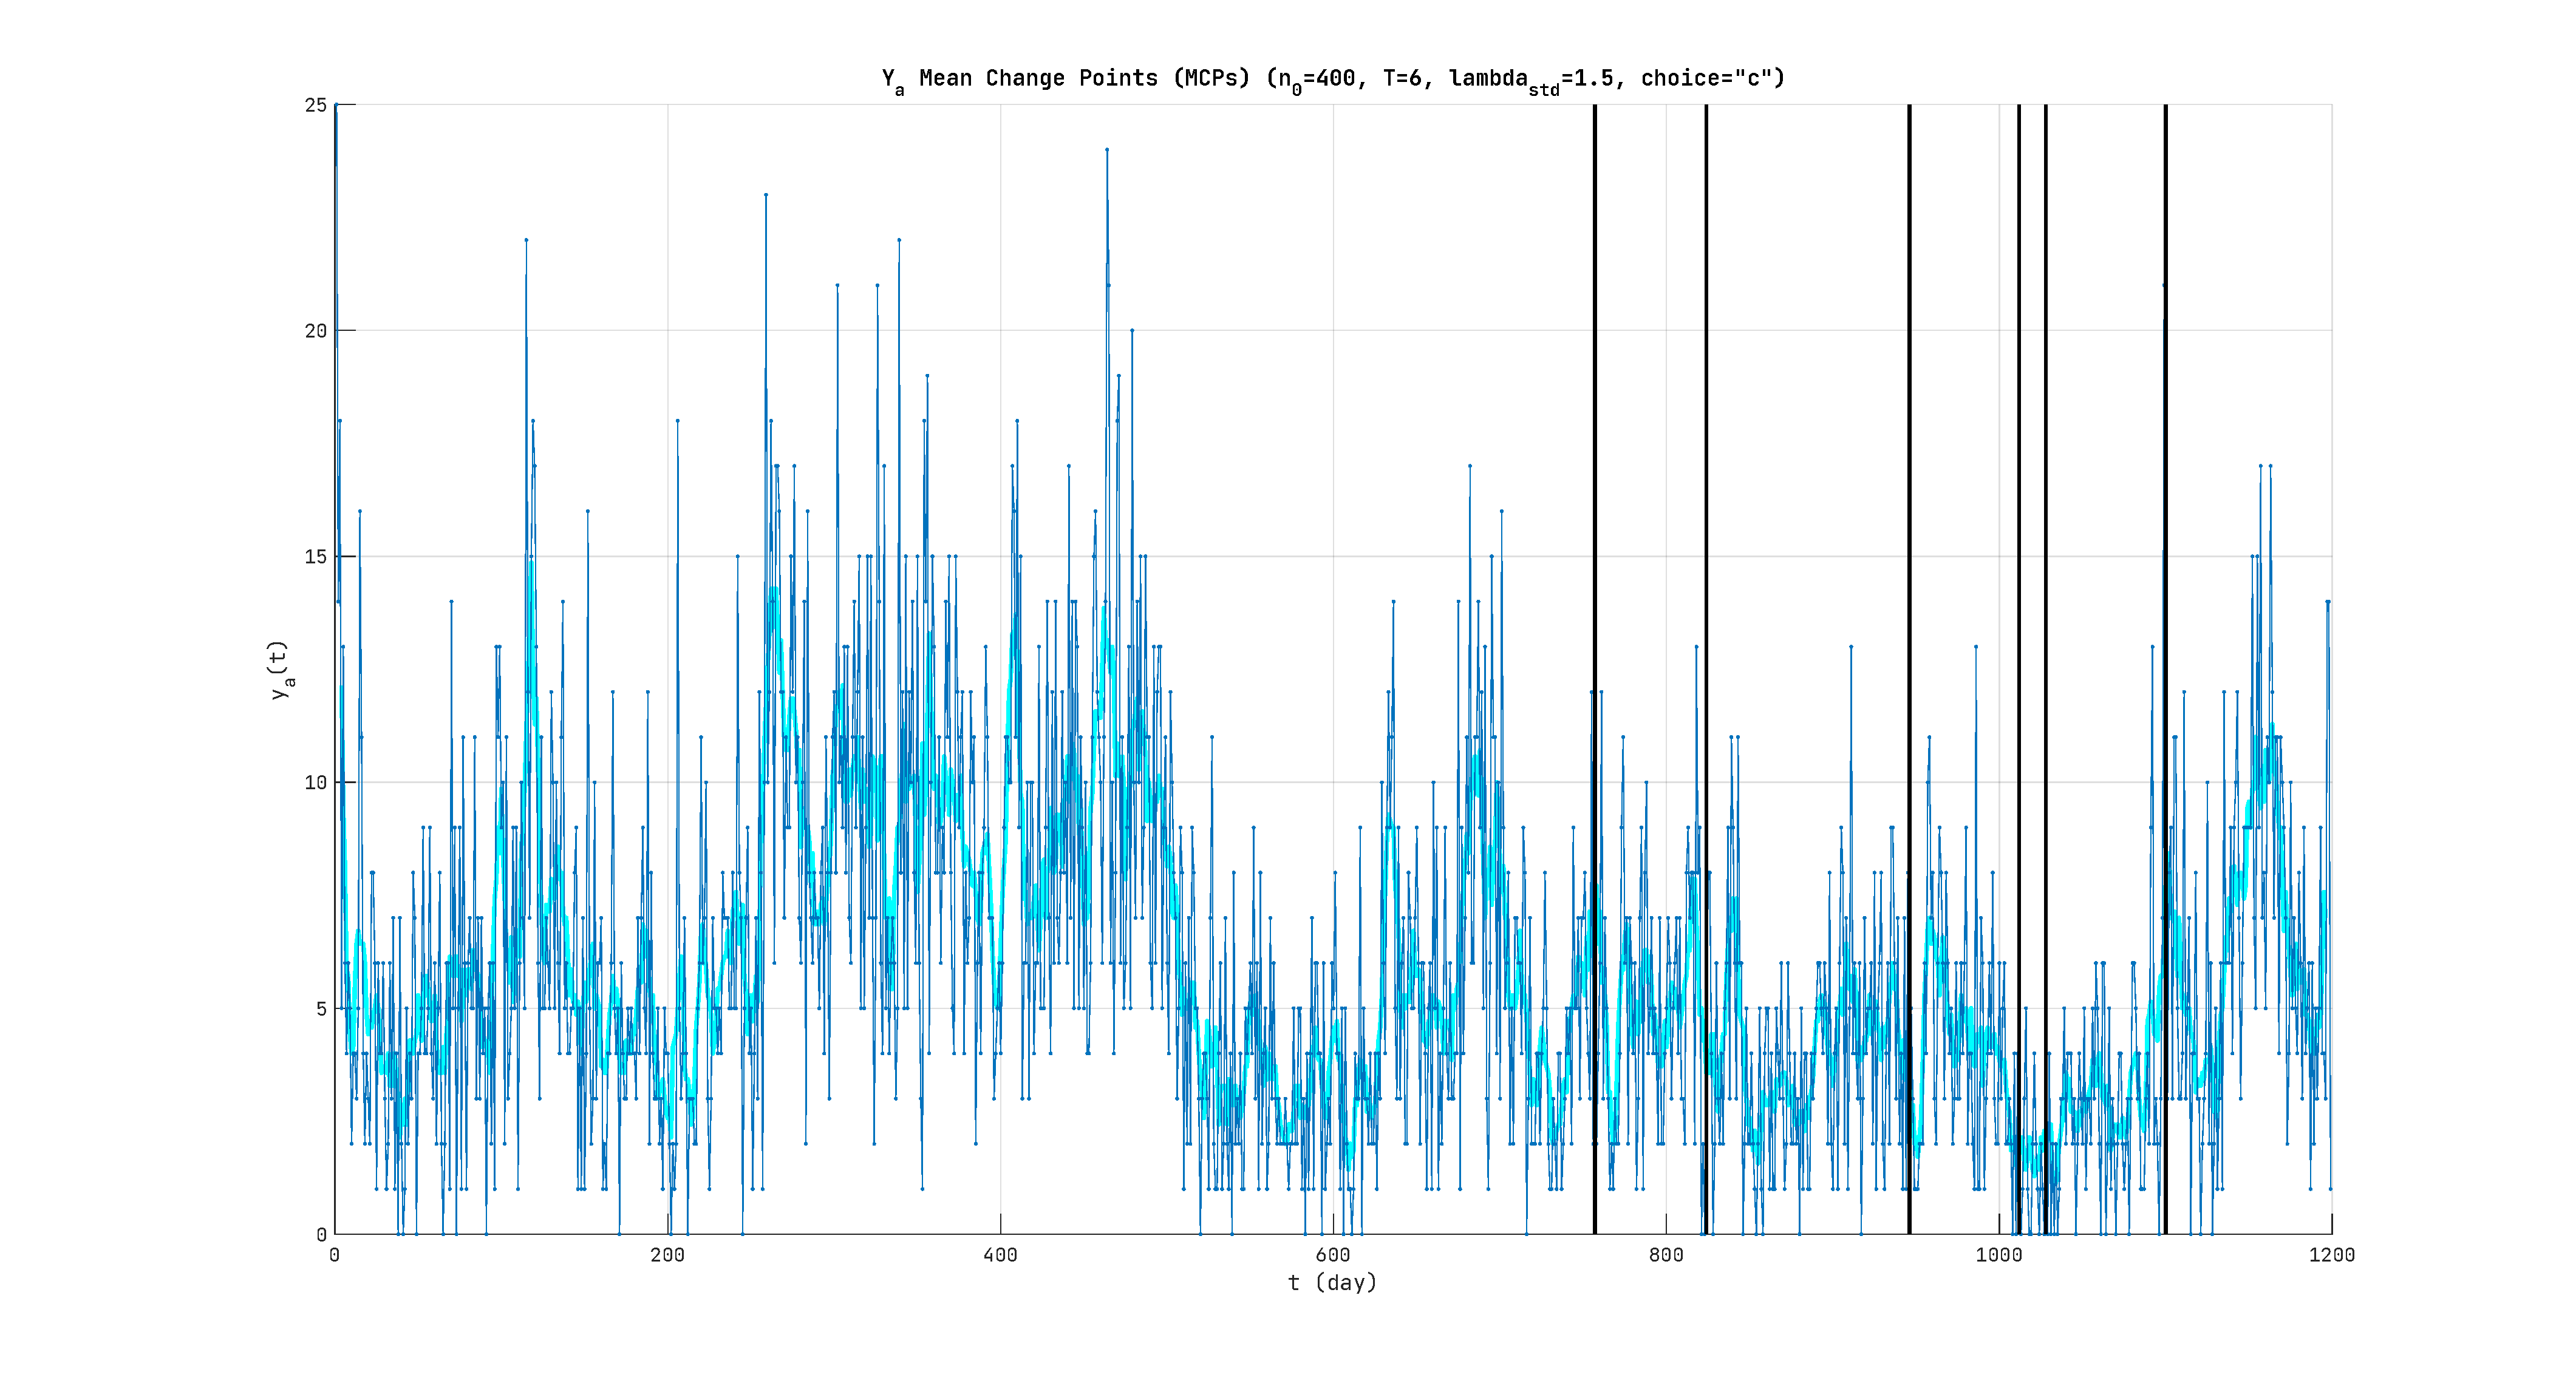
\includegraphics[width=\textwidth]{plots/mcps_ya_opt_c.svg.pdf}
        \caption{Διάγραμμα ιστορίας της αρχικής χρονοσειράς $\{Y_a(t)\}$ (μπλε) μαζί με τα σημεία αλλαγής (μαύρο) που επιλέχθηκαν από την ανάλυση της στάσιμης εκδοχής της με τις βέλτιστες παραμέτρους, καθώς και εκτίμηση της τάσης με φίλτρο κινούμενου μέσου τάξης 7 ($MA(7)$ \tl{smoothing}) - επιλογή \textquote{\tl{c}}}
        \label{fig:mcps_ya_opt_c}
    \end{center}
\end{figure}


\subsection{Αναπροσαρμογή σε κάθε χρονική στιγμή}

Επιλογή \textquote{\tl{b}}

\par Τα ίδια διαγράμματα παρουσιάζονται για την επιλογή αναπροσαρμογής \textquote{\tl{b}} (αναπροσαρμογή σε κάθε χρονική στιγμή) ενώ ακολουθεί σύντομος σχολιασμός:

\begin{figure}[H]
    \begin{center}
        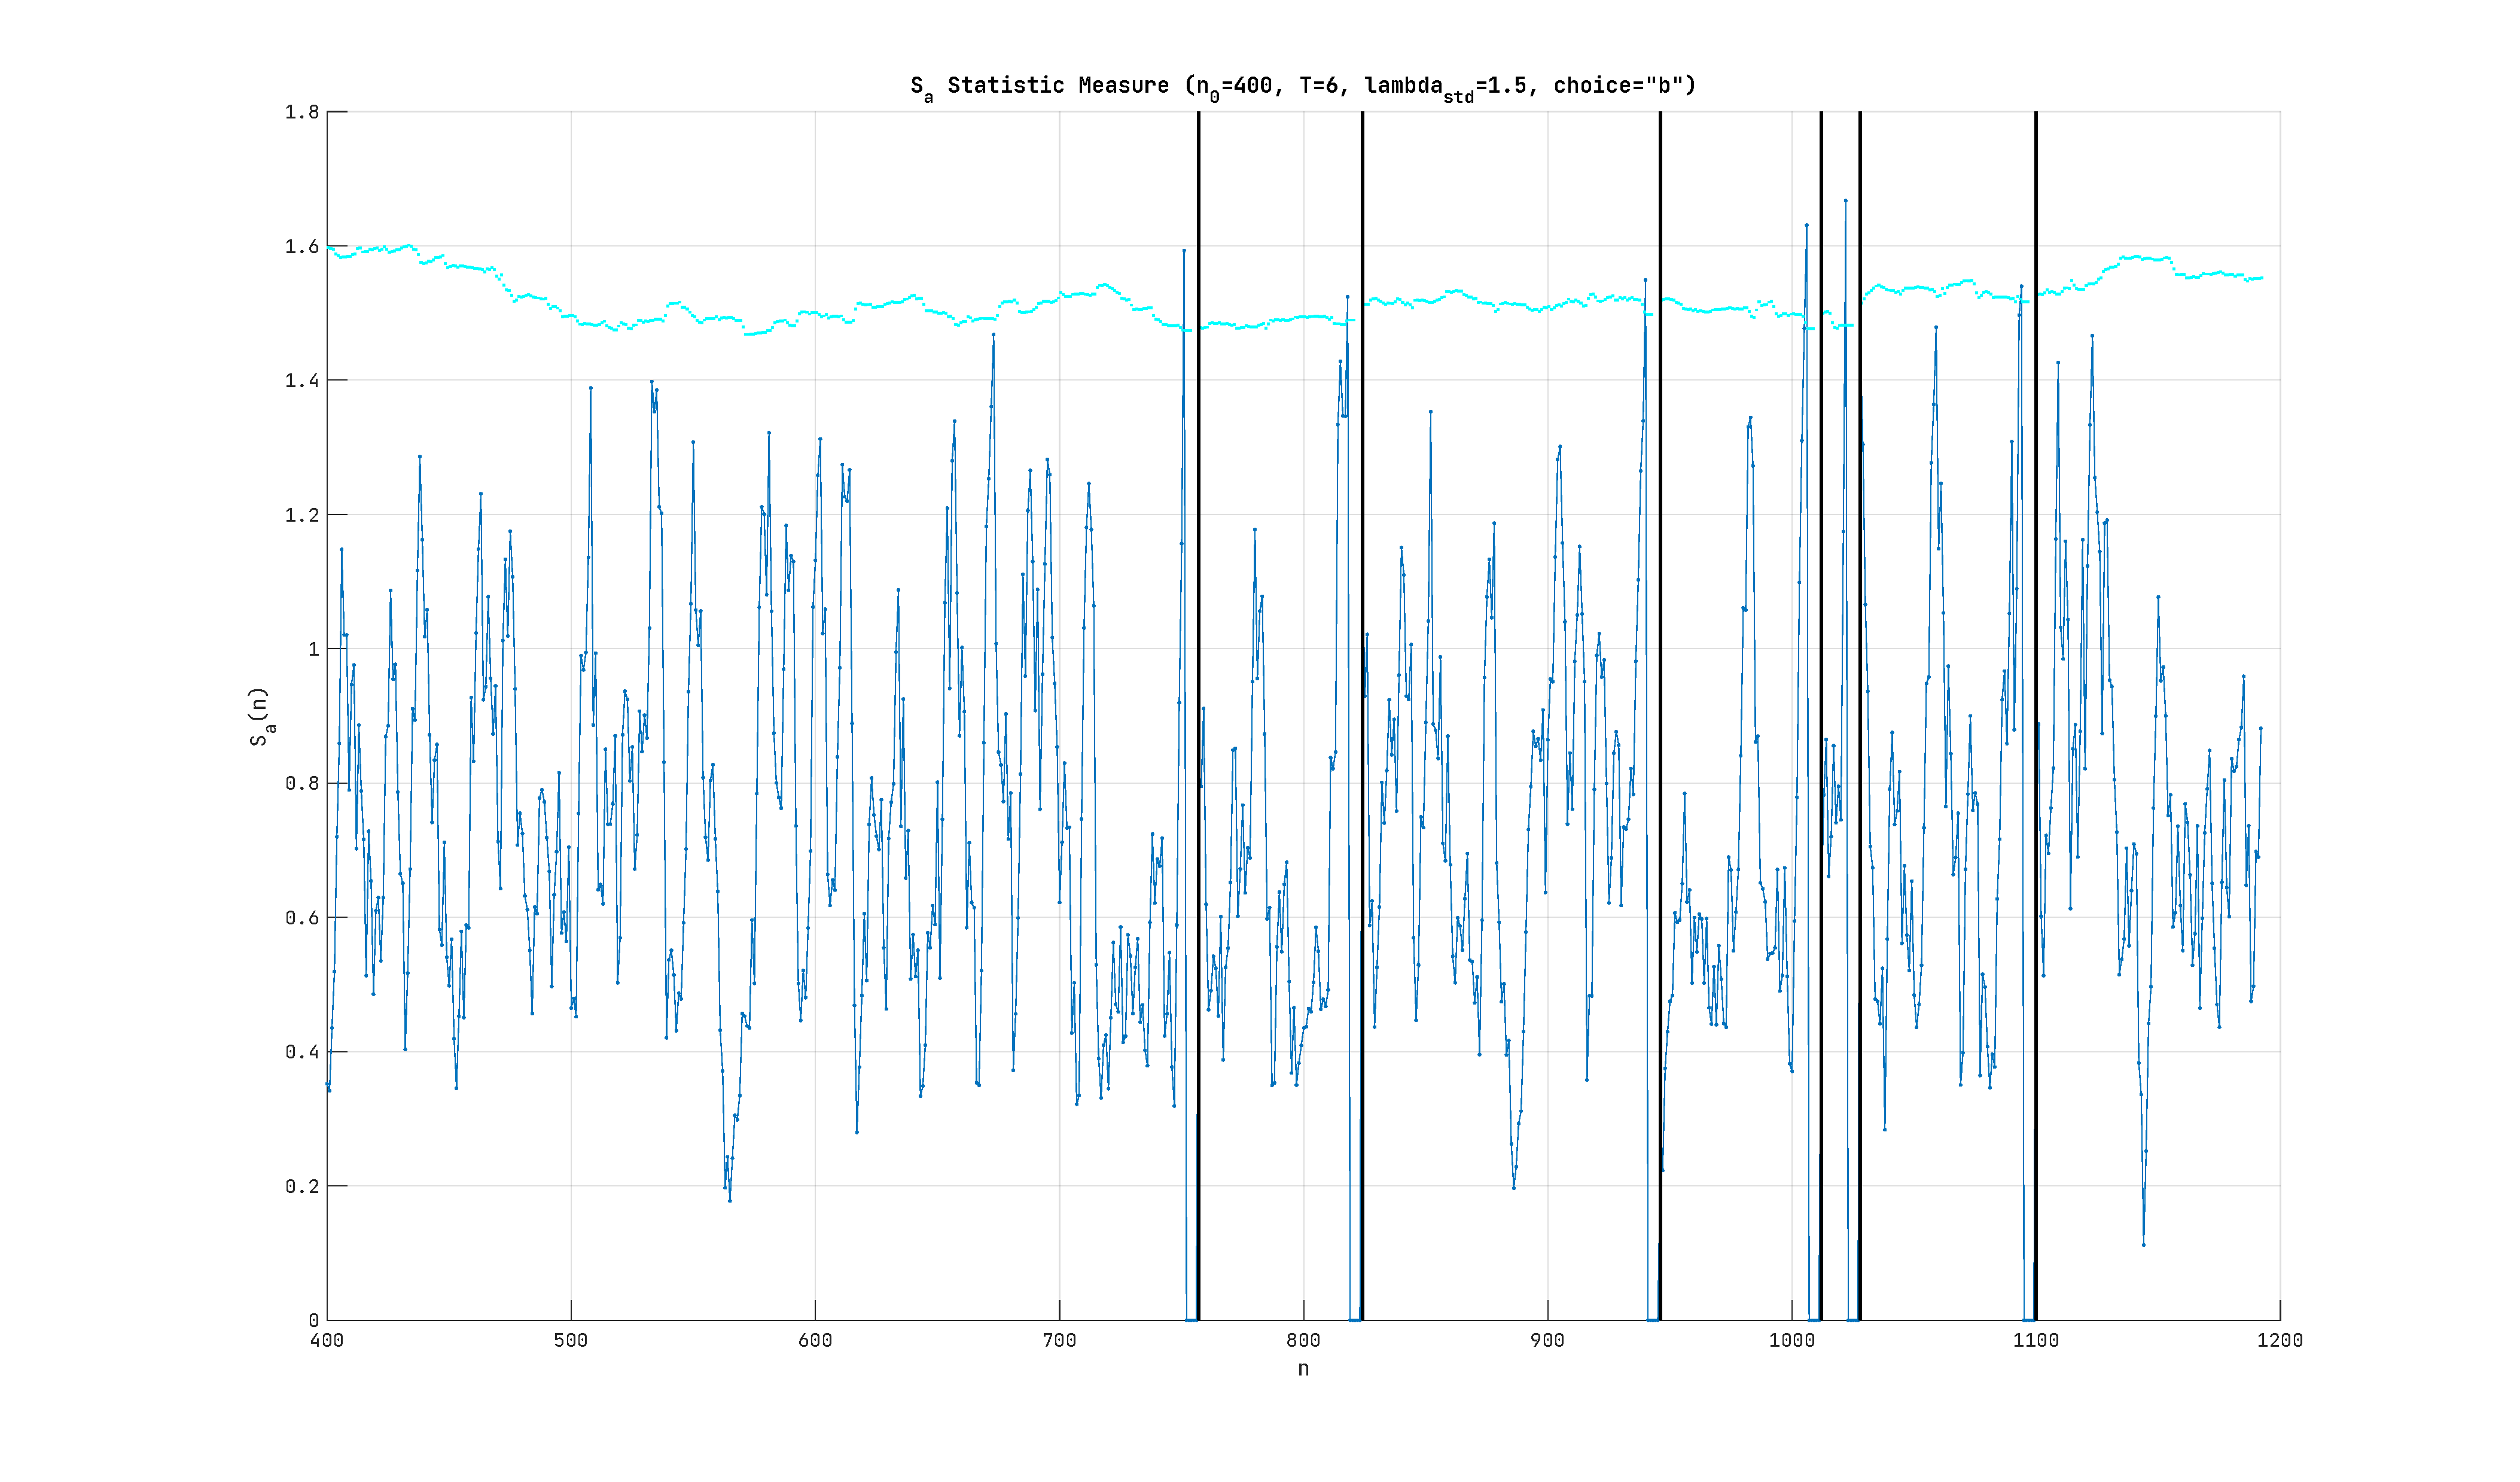
\includegraphics[width=\textwidth]{plots/mcps_xa_opt_b.svg.pdf}
        \caption{Τιμές στατιστικού $S_n$ για έως και 6 βήματα μπροστά πρόβλεψη με $MA(1)$ της στάσιμης χρονοσειράς $\{X_a(t)\}$ και για επιλογή αναπροσαρμογής \textquote{\tl{b}} (αναπροσαρμογή σε κάθε χρονική στιγμή). Σημειώνονται επίσης το κριτήριο απόφασης, $\alpha=1.5*s_x$, (\tl{cyan}) και φυσικά τα σημεία αλλαγής με έντονες κάθετες γραμμές στα εκάστοτε σημεία $n+T$ (μαύρο) - [\tl{NRMSE}=0.802, \ 86.1\tl{sec}]}
        \label{fig:mcps_xa_opt_b}
    \end{center}
\end{figure}

Παρακάτω, τα ίδια σημεία αλλαγής απεικονίζονται στην αρχική χρονοσειρά προβολών του βίντεο \tl{A}:

\begin{figure}[H]
    \begin{center}
        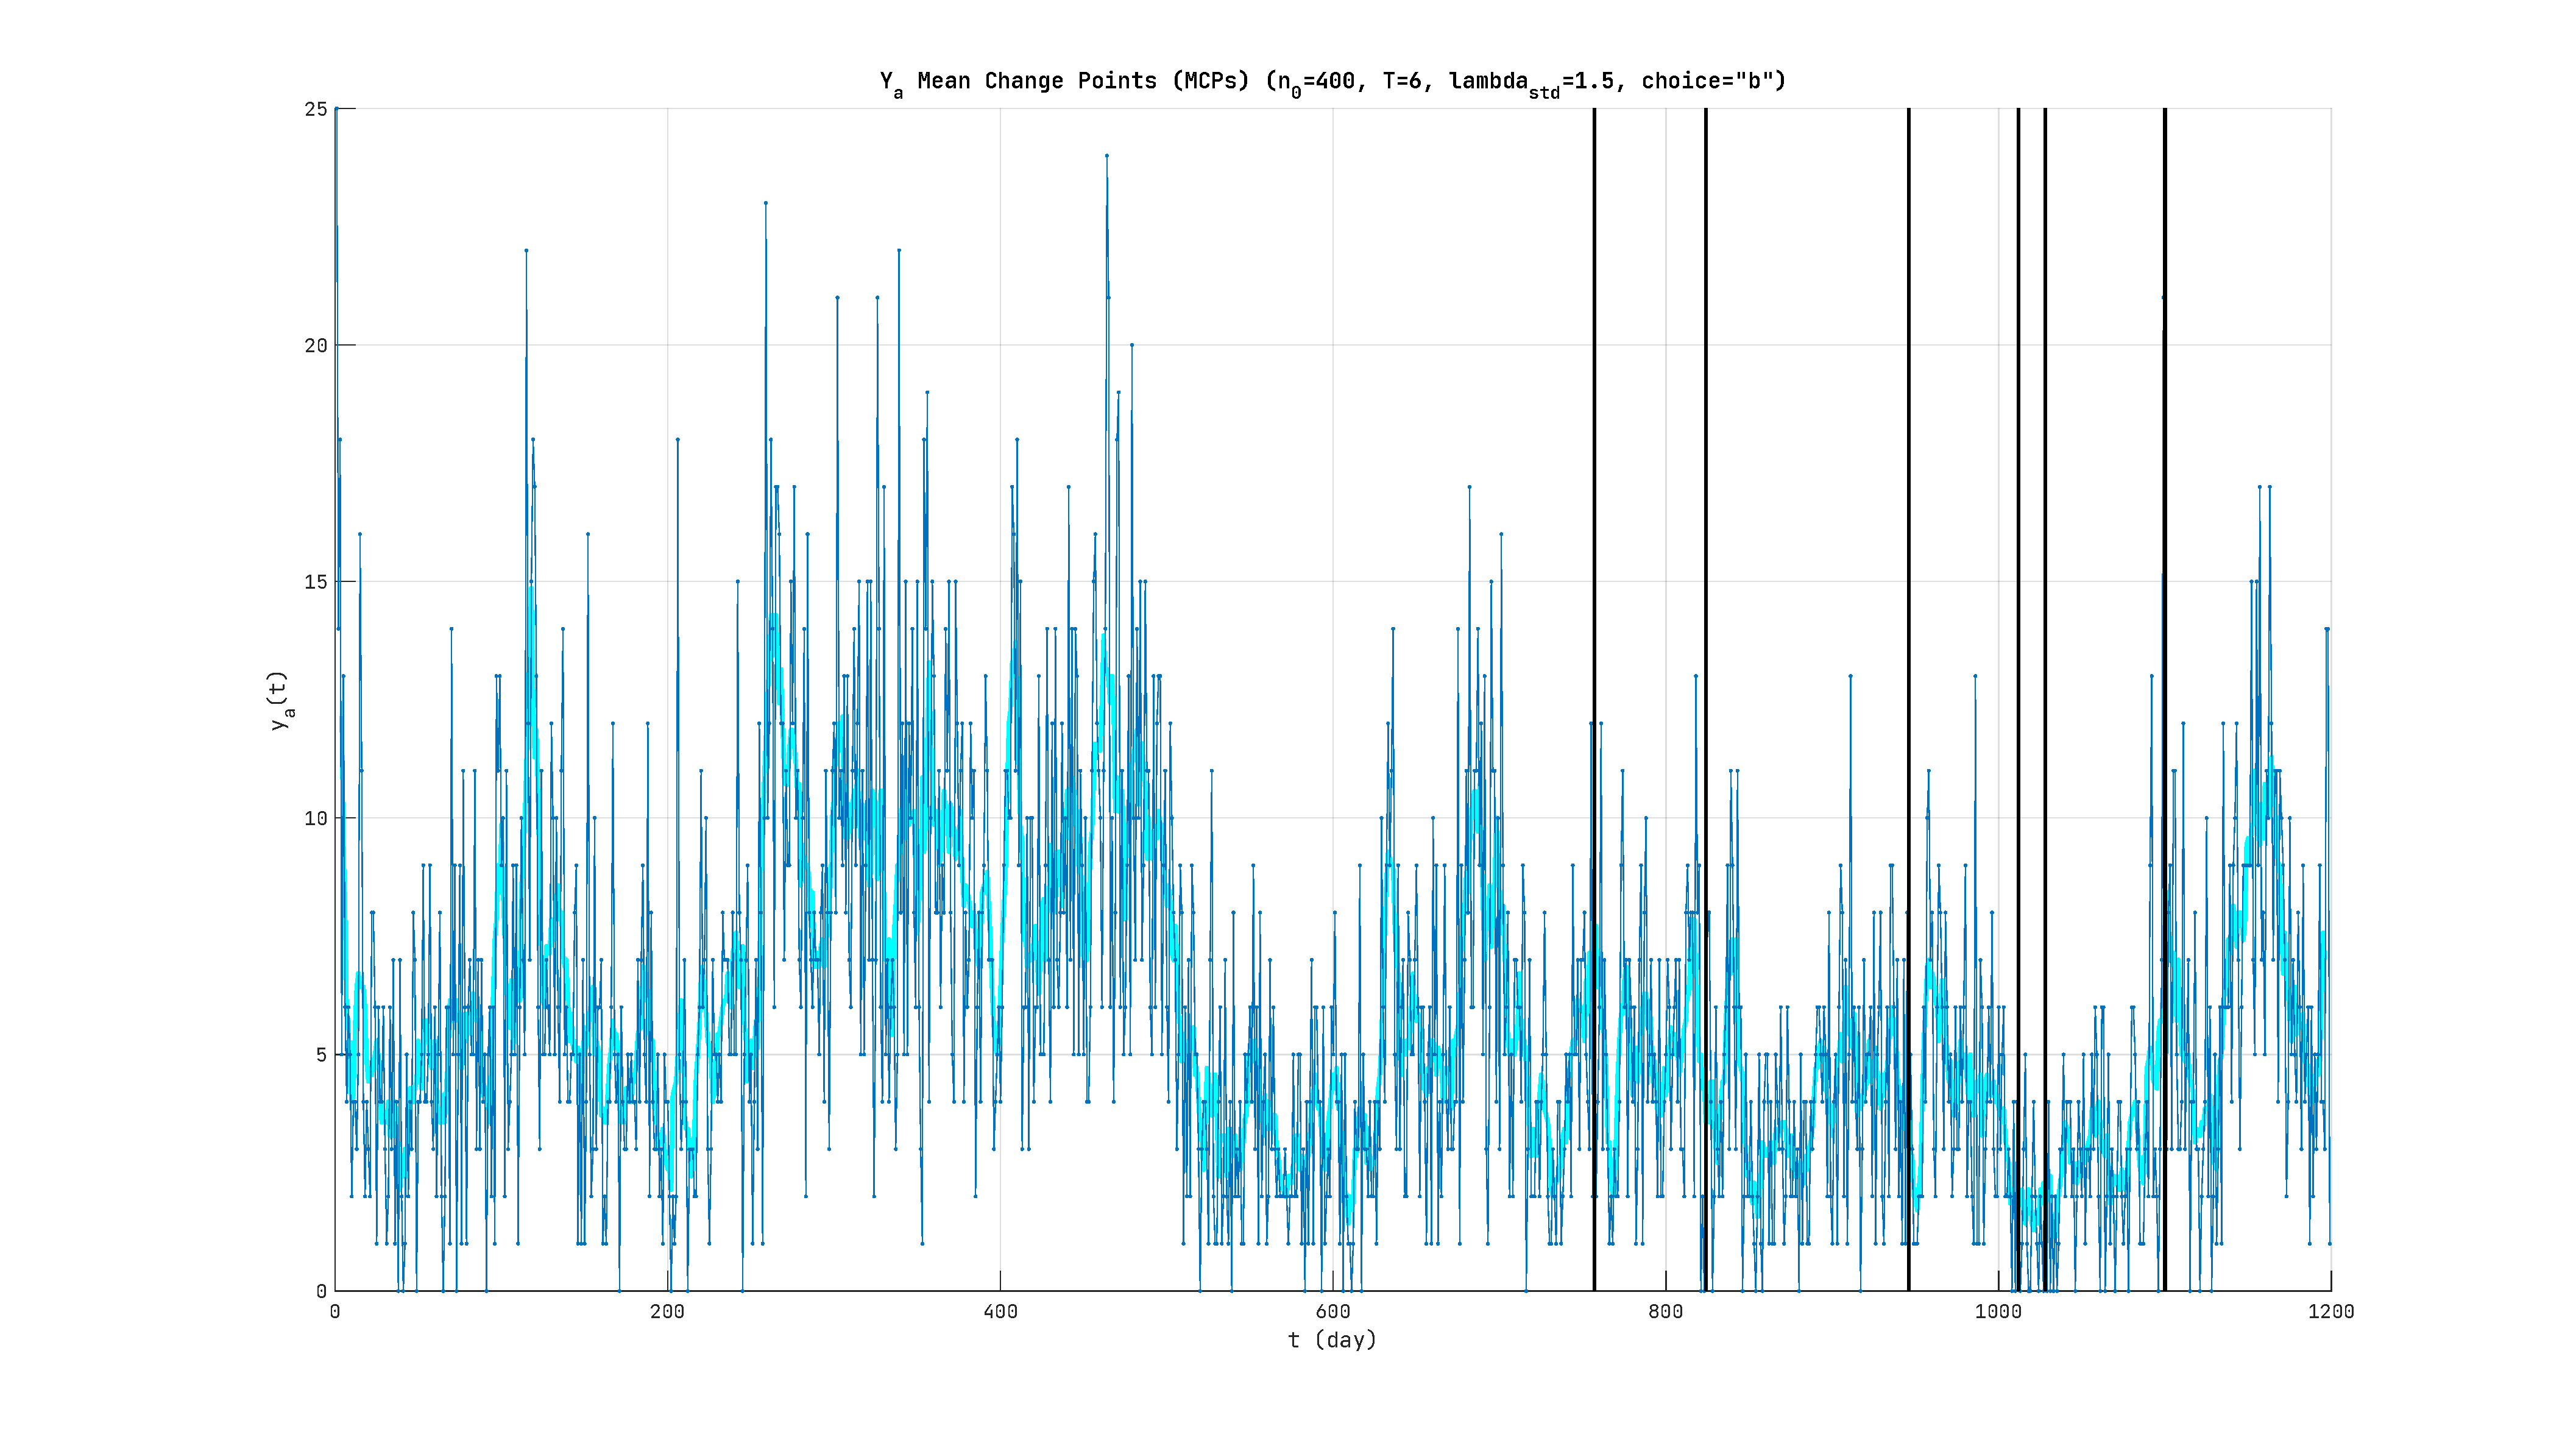
\includegraphics[width=\textwidth]{plots/mcps_ya_opt_b.svg.pdf}
        \caption{Διάγραμμα ιστορίας της αρχικής χρονοσειράς $\{Y_a(t)\}$ (μπλε) μαζί με τα σημεία αλλαγής (μαύρο) που επιλέχθηκαν από την ανάλυση της στάσιμης εκδοχής της με τις βέλτιστες παραμέτρους, καθώς και εκτίμηση της τάσης με φίλτρο κινούμενου μέσου τάξης 7 ($MA(7)$ \tl{smoothing}) - επιλογή \textquote{\tl{b}}}
        \label{fig:mcps_ya_opt_b}
    \end{center}
\end{figure}

Βλέποντας τα τελευταία δύο (2) διαγράμματα και συγκρίνοντάς τα με αυτά της επιλογής \textquote{\tl{c}} κάνουμε τις εξής παρατηρήσεις:
\begin{enumerate}
    \item Τα σημεία αλλαγής είναι ίδια σε αριθμό (6) και μάλιστα στις ακριβώς ίδιες θέσεις (με εξαίρεση το τελευταίο που έχει μετατοπιστεί 2 χρονικές στιγμές μετά)
    \item Το όριο απόφασης (\tl{cyan} διακεκομμένη γραμμή) φαίνεται να έχει πολύ μεγαλύτερη διακύμανση σε σύγκριση με αυτό της επιλογής \textquote{\tl{c}}, κάτι απολύτως αναμενόμενο αφού η αναπροσαρμογή γίνεται πλέον σε κάθε βήμα / χρονική στιγμή και άρα αντίστοιχα η δειγματική τυπική απόκλιση των παρατηρήσεων του \tl{training set} αλλάζει συνεχώς
\end{enumerate}


\subsection{Χωρίς Αναπροσαρμογή}

\par Τέλος, τα ίδια διαγράμματα παρουσιάζονται για την επιλογή αναπροσαρμογής \textquote{\tl{a}} (καμία αναπροσαρμογή - διατήρηση του μοντέλου που προσαρμόστηκε στις πρώτες 400 παρατηρήσεις της στάσιμης χρονοσειράς), ενώ ακολουθεί σύντομος σχολιασμός:

\begin{figure}[H]
    \begin{center}
        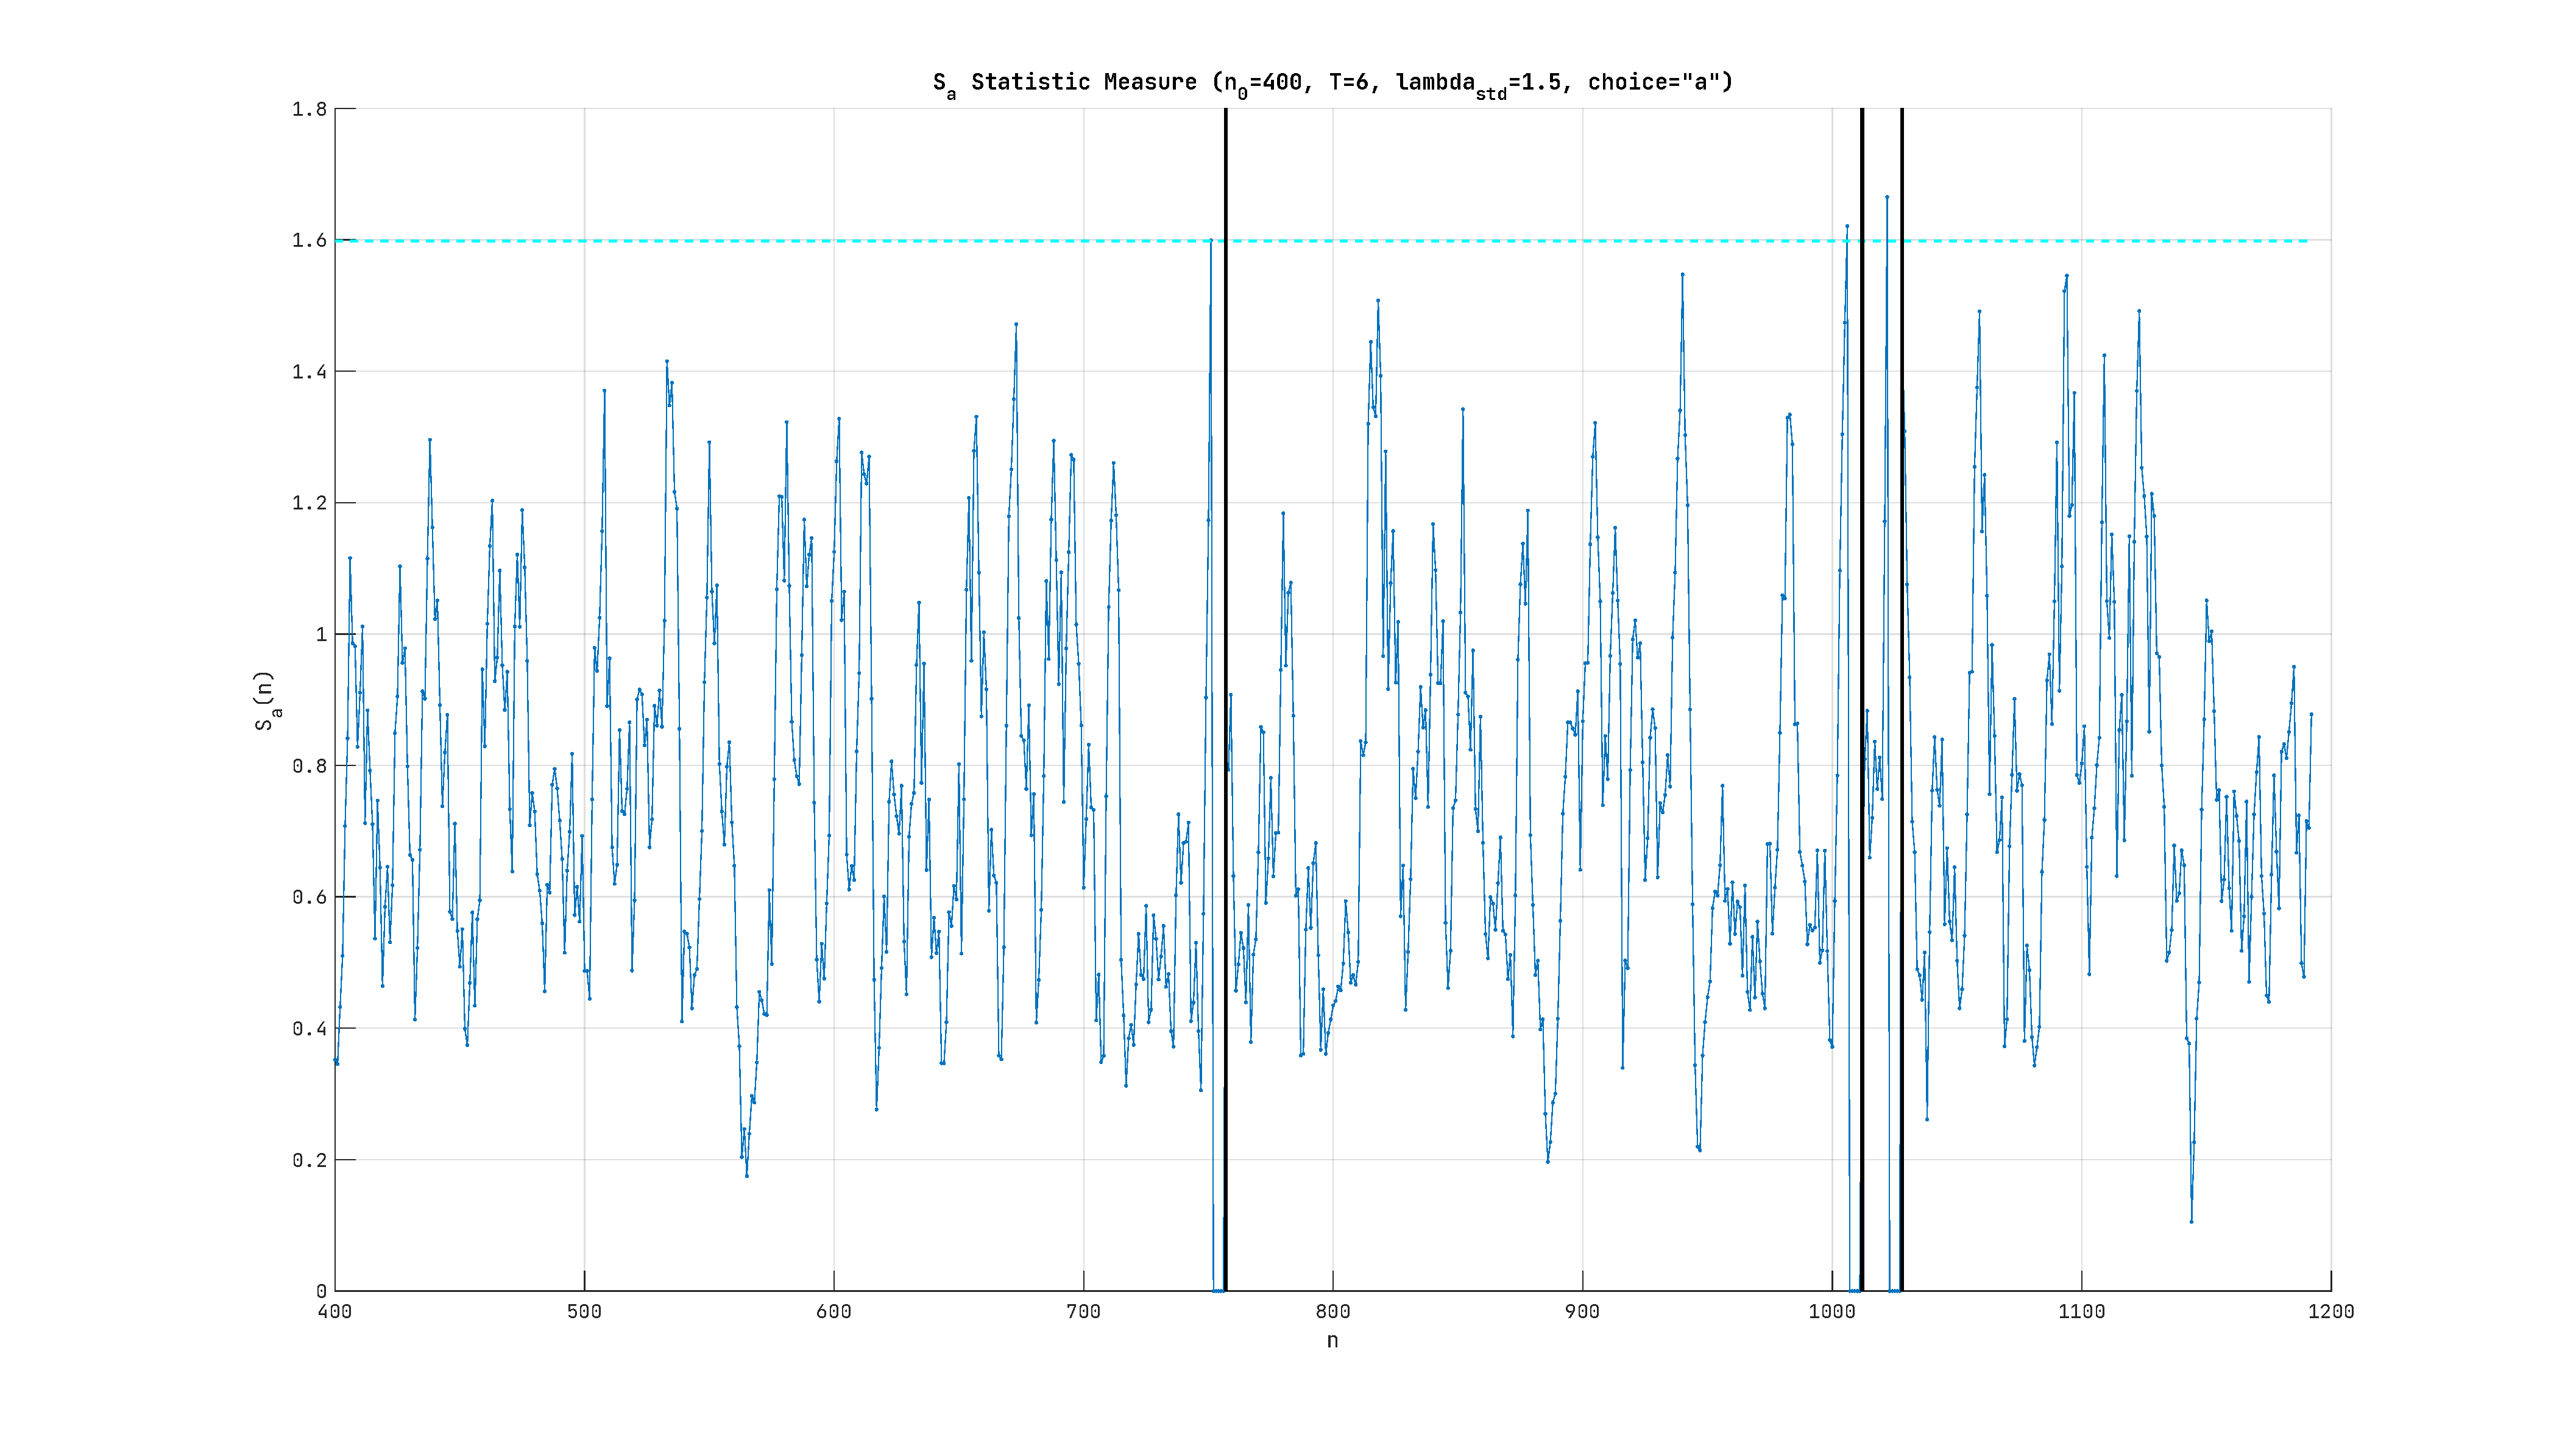
\includegraphics[width=\textwidth]{plots/mcps_xa_opt_a.svg.pdf}
        \caption{Τιμές στατιστικού $S_n$ για έως και 6 βήματα μπροστά πρόβλεψη με $MA(1)$ της στάσιμης χρονοσειράς $\{X_a(t)\}$ και για επιλογή αναπροσαρμογής \textquote{\tl{a}} (χωρίς αναπροσαρμογή). Σημειώνονται επίσης το κριτήριο απόφασης, $\alpha=1.5*s_x$, (\tl{cyan}) και φυσικά τα σημεία αλλαγής με έντονες κάθετες γραμμές στα εκάστοτε σημεία $n+T$ (μαύρο) - [\tl{NRMSE}=0.789, \ 27.2\tl{sec}]}
        \label{fig:mcps_xa_opt_a}
    \end{center}
\end{figure}

Παρακάτω, τα ίδια σημεία αλλαγής απεικονίζονται στην αρχική χρονοσειρά προβολών του βίντεο \tl{A}:

\begin{figure}[H]
    \begin{center}
        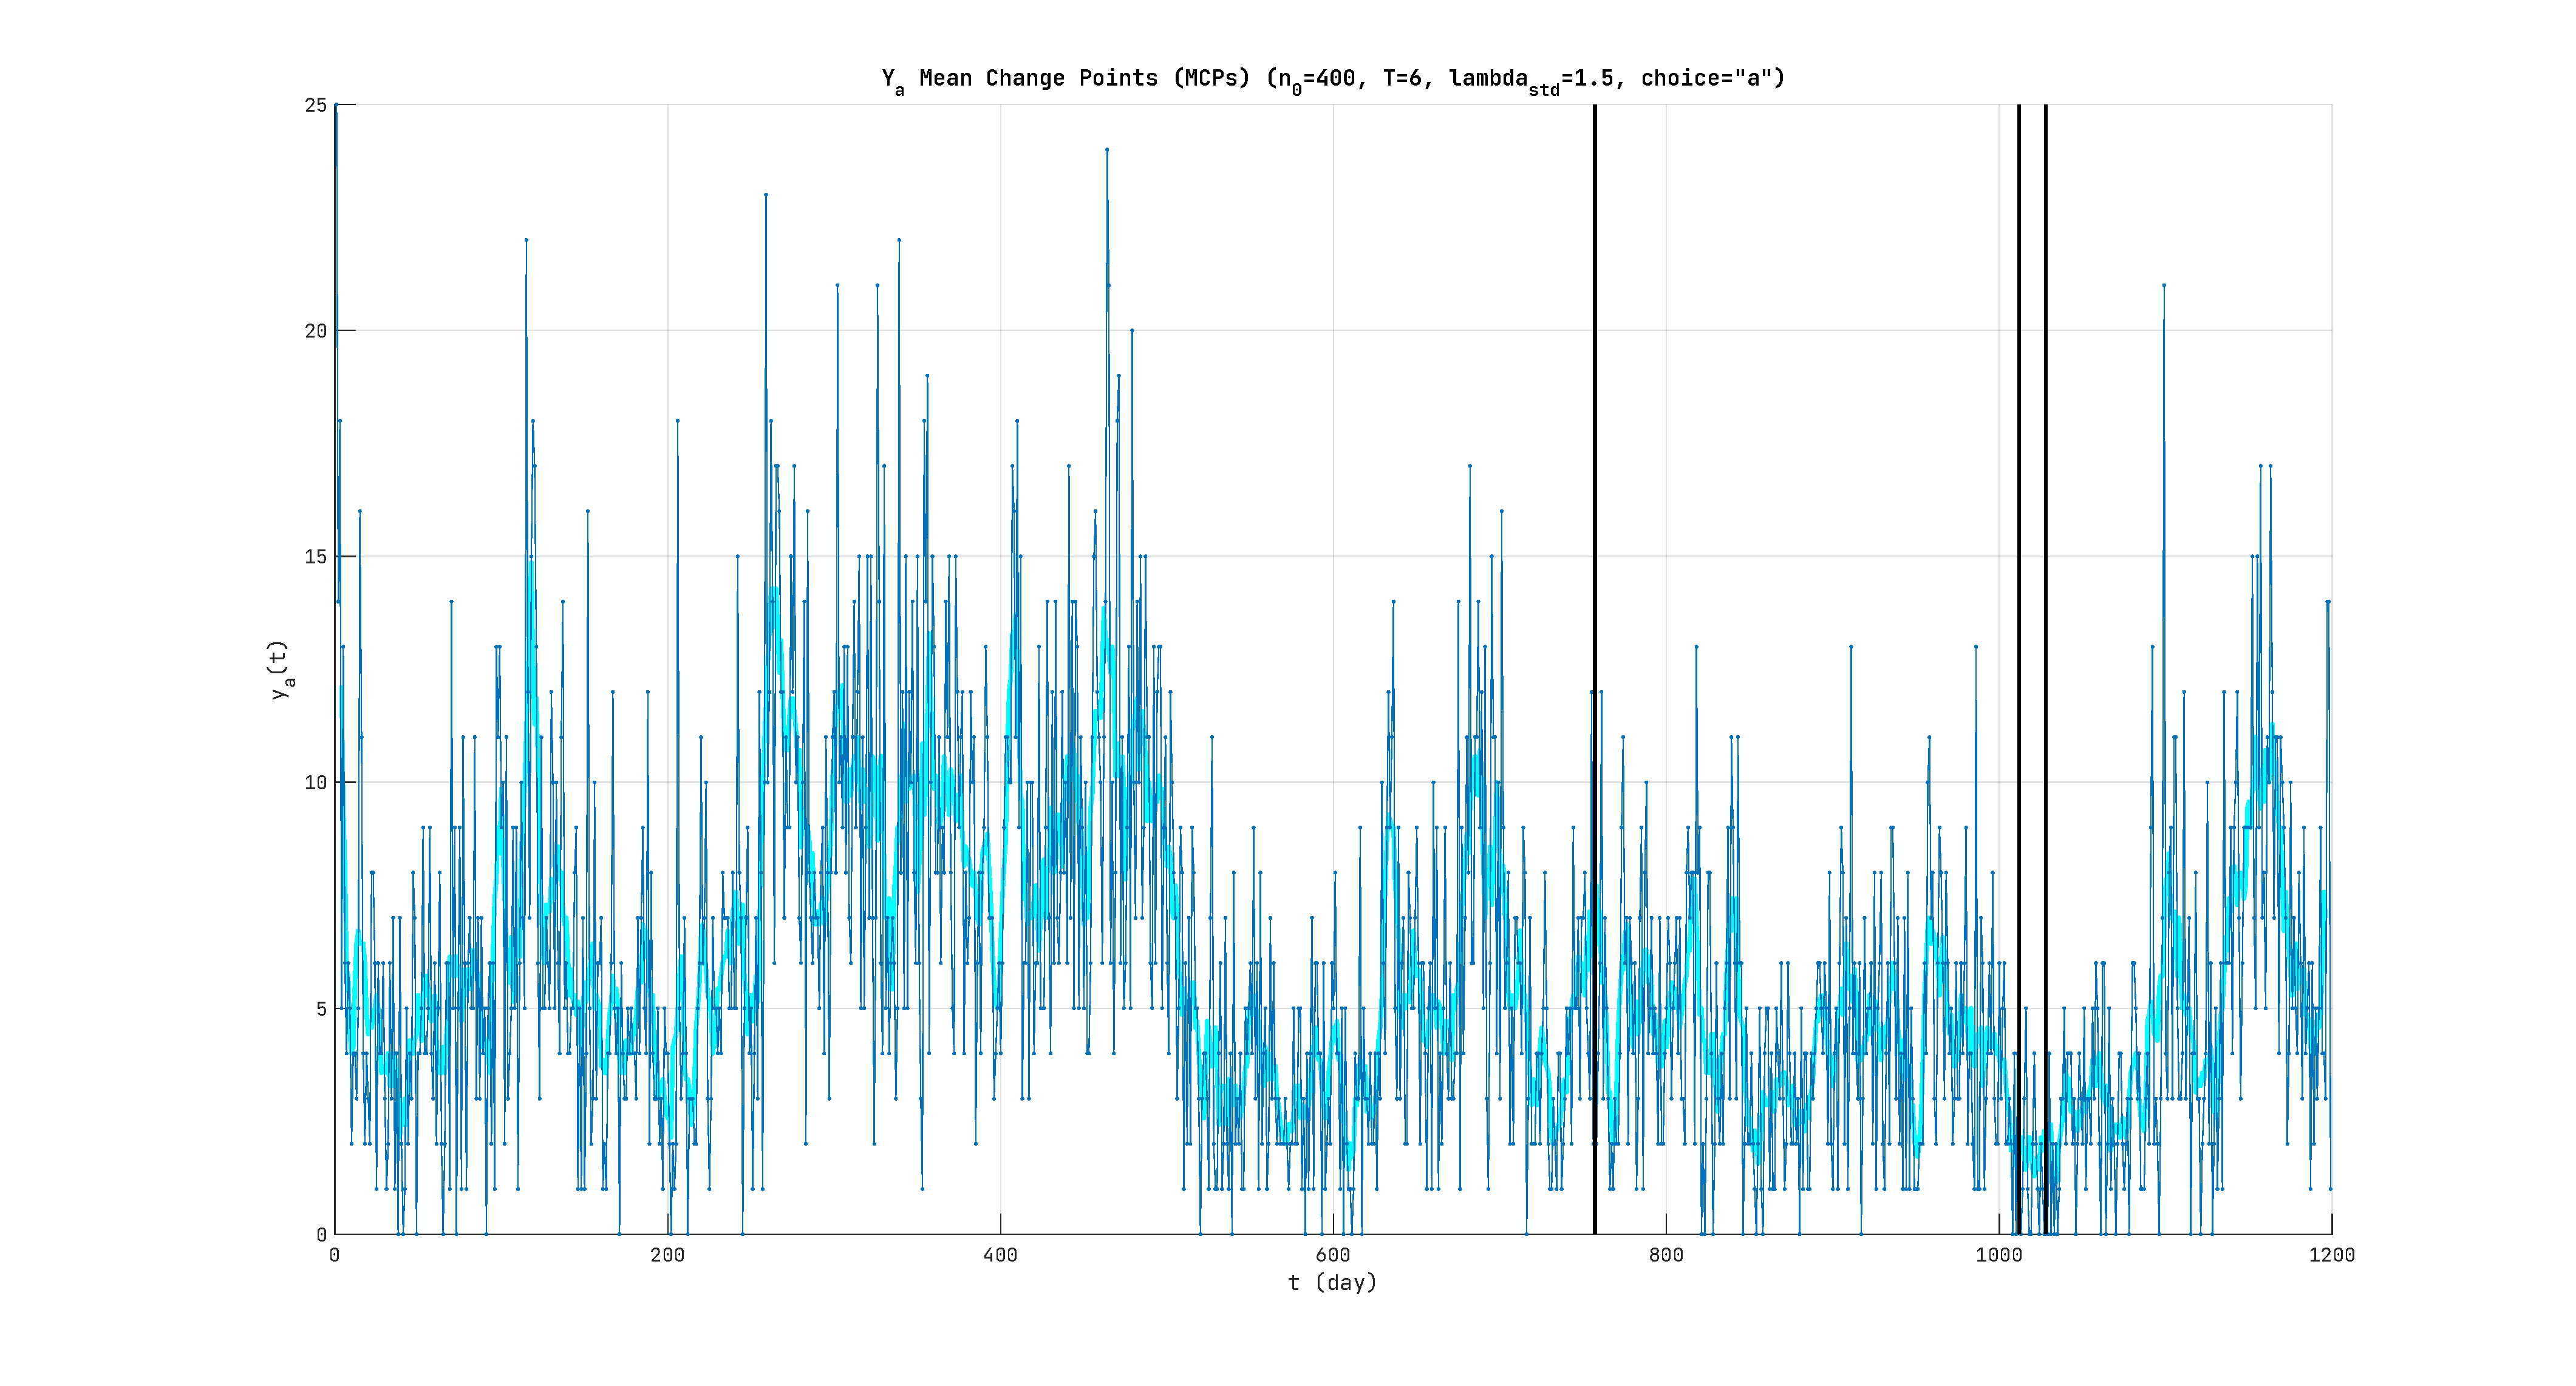
\includegraphics[width=\textwidth]{plots/mcps_ya_opt_a.svg.pdf}
        \caption{Διάγραμμα ιστορίας της αρχικής χρονοσειράς $\{Y_a(t)\}$ (μπλε) μαζί με τα σημεία αλλαγής (μαύρο) που επιλέχθηκαν από την ανάλυση της στάσιμης εκδοχής της με τις βέλτιστες παραμέτρους, καθώς και εκτίμηση της τάσης με φίλτρο κινούμενου μέσου τάξης 7 ($MA(7)$ \tl{smoothing}) - επιλογή \textquote{\tl{a}}}
        \label{fig:mcps_ya_opt_a}
    \end{center}
\end{figure}

Βλέποντας τα τελευταία δύο (2) διαγράμματα και συγκρίνοντάς τα με αυτά της επιλογής \textquote{\tl{c}} κάνουμε τις εξής παρατηρήσεις:
\begin{enumerate}
    \item Τα σημεία αλλαγής είναι λιγότερα, πλέον μόλις τρία (3) αλλά αυτά τα τρία βρίσκονται στις ακριβώς ίδιες θέσεις με τα αντίστοιχα. Αυτό οφείλεται στο ότι το όριο επιλογής παραμένει σταθερό παρόλο που η τυπική απόκλιση των δειγμάτων αλλάζει καθώς προχωράμε στη στάσιμη χρονοσειρά πράγμα που φαίνεται και από το αντίστοιχο διάγραμμα της επιλογής \textquote{\tl{b}}
    \item Το όριο απόφασης (\tl{cyan} διακεκομμένη γραμμή), όπως αναφέρθηκε, παραμένει συνεχώς σταθερό, κάτι πιθανότατα μη επιθυμητό
\end{enumerate}

Καταληκτικά, η πιο κατάλληλη επιλογή για αναπροσαρμογή του μοντέλου πρόβλεψης είναι η επιλογή \textquote{\tl{c}} (αναπροσαρμογή όταν βρεθεί σημείο αλλαγής) καθώς συνδυάζει καλή υπολογιστική συμπεριφορά αλλά ταυτόχρονα εξασφαλίζει και ότι το μοντέλο και άρα και το όριο επιλογής σημείων αλλαγής μεταβάλλεται καθώς προχωράμε στη χρονοσειρά και βρίσκουμε σημεία αλλαγής. Πρέπει να σημειωθεί επίσης ότι αυτή η επιλογή χρησιμοποιήθηκε και κατά το \tl{grid search} των \tl{hyperparameters} (σχήματα \ref{fig:mcps_count_a} και \ref{fig:nrmse_a} παραπάνω).